\documentclass[11pt,a4paper]{report}

% --- Essential packages ---
\usepackage[utf8]{inputenc}
\usepackage[T1]{fontenc}
\usepackage{lmodern}
\usepackage[french]{babel}
\usepackage{csquotes}

% --- Layout and spacing ---
\usepackage{geometry}
\usepackage{setspace}
\usepackage{titlesec}
\usepackage{fancyhdr}
\usepackage{xcolor}

% --- Math and symbols ---
\usepackage{amsmath, amssymb}
\usepackage{textcomp}

% --- Lists and tables ---
\usepackage{enumitem}
\usepackage{booktabs}
\usepackage{tabularx}
\usepackage{multirow}
\usepackage{array}

% --- Graphics and links ---
\usepackage{graphicx}
\usepackage{placeins}
\usepackage{float}
\usepackage{caption}
\usepackage{microtype}
\DisableLigatures[-]{encoding=T1,family=tt*} % keep "--option" as two hyphens in \code
\usepackage[hidelinks]{hyperref}
\setlength{\emergencystretch}{3em}

% --- Bibliography ---
% backend=bibtex : compile sans biber (localement et sur Overleaf).
\usepackage[backend=bibtex, style=ieee]{biblatex}
\addbibresource{references.bib}
% Le style ieee n'a pas de traduction française pour le numéro d'article (champ eid).
\DefineBibliographyStrings{french}{artno = {art.~n\textsuperscript{o}}}

% --- Helpers ---
\newcommand{\code}[1]{\texttt{\detokenize{#1}}}
\newcommand{\todo}[1]{\textcolor{red}{[TODO : #1]}}
\newcolumntype{Y}{>{\raggedright\arraybackslash}X}

% Page margins
\geometry{left=3cm, right=2.5cm, top=2.5cm, bottom=2.5cm}

% Header / Footer
\pagestyle{fancy}
\fancyhf{}
\fancyfoot[C]{MSE Travail de Master -- Estimation de pose dans psifx}
\fancyfoot[R]{\thepage}
\renewcommand{\headrulewidth}{0pt}
\renewcommand{\footrulewidth}{0.4pt}

% Line spacing
\onehalfspacing

% Title formatting
\titleformat{\chapter}[hang]{\bfseries\Huge}{\thechapter.}{2pc}{}
\titleformat{\section}[hang]{\bfseries\Large}{\thesection}{1em}{}

\begin{document}

% =============================================================================
% Page de titre
% =============================================================================
\begin{titlepage}
    \centering

    % Logos (optionnels : ajoutes s'ils sont presents dans images/)
    \IfFileExists{images/mse_logo.png}{%
    \begin{minipage}[t]{0.49\textwidth}
        \includegraphics[height=2cm]{images/mse_logo.png}
    \end{minipage}}{}
    \hfill
    \IfFileExists{images/hes_logo.png}{%
    \begin{minipage}[t]{0.49\textwidth}
        \raggedleft
        \includegraphics[height=2cm]{images/hes_logo.png}
    \end{minipage}}{}

    \vspace*{2cm}
    {\Large Master of Science HES-SO in Engineering} \\[0.2cm]
    Av. de Provence 6 \\
    CH-1007 Lausanne \\[2cm]

    {\Large Orientation : Computer Science (CS)}\\[1.5cm]

    {\Huge\bfseries Estimation de pose humaine dans psifx :\\[0.3cm]
    choisir, intégrer et optimiser des modèles récents\\[1cm]}

    {\Large Travail de Master -- Rapport, version 1}\\[2cm]

    {\large Andy Montaru}\\[1cm]

    \begin{tabular}{rl}
        Professeur responsable : & Calbimonte Jean Paul \\
        Expert externe / contact psifx : & Matthew Vowels (UNIL) \\
    \end{tabular}

    \vfill
    {\large Lausanne, \today}
\end{titlepage}

% =============================================================================
% Résumé
% =============================================================================
\chapter*{Résumé}
\addcontentsline{toc}{chapter}{Résumé}

psifx \cite{psifx2024} est une bibliothèque Python d'extraction de caractéristiques destinée à la recherche en
sciences humaines (interactions sociales filmées). Son unique backend d'estimation de pose humaine, MediaPipe, est
léger mais nettement moins précis que les modèles récents. Ce travail cherche à choisir de manière objective et
reproductible quel(s) modèle(s) intégrer à psifx, en tenant compte non seulement de la précision, mais aussi de la
stabilité temporelle, du coût de calcul, de la licence et de la cohérence avec l'architecture existante.

Après une revue de l'état de l'art (modèles de pose 2D, segmentation et suivi vidéo, méthodologies de mesure de
précision, littérature en sciences du comportement), un banc de mesure reproductible a été construit sur un
sous-ensemble de COCO \cite{lin2014coco} et une vidéo d'interaction. Huit configurations ont été comparées :
MediaPipe, RTMPose, RTMO, DETRPose, ViTPose et trois tailles de Sapiens2. MediaPipe obtient un OKS moyen de 0,235,
contre 0,830 à 0,890 pour les meilleurs candidats ; Sapiens2 reste impraticable en vidéo (0,9 à 1,3 image/s).

Quatre modèles (RTMPose, RTMO, ViTPose, DETRPose) ont ensuite été intégrés à psifx comme remplaçants directs de
MediaPipe, chacun dans sa propre branche, avec des tests unitaires et un test de non-régression de précision sur
COCO. Des optimisations d'inférence (fp16, \code{torch.compile}, quantification INT8) ont été mesurées sur chacun.
Le meilleur gain est obtenu par RTMO en fp16 (+43\,\%, 110 images/s, précision inchangée) ; l'INT8 statique s'est
révélé à la fois plus lent et nettement moins précis sur ce matériel. Le profilage montre que, pour ViTPose et
DETRPose, le modèle lui-même ne représente qu'une minorité du temps : les vrais leviers sont le détecteur, le
prétraitement et, pour DETRPose, le pont entre environnements Python.

Une seconde phase a approfondi ces résultats et testé psifx de bout en bout. L'écart de ViTPose s'explique par le
détecteur et n'est pas significatif ; l'échec de l'INT8 vient d'une erreur cumulée dans le modèle de pose et de
convolutions que l'activation SiLU empêche de fusionner. RTMO et ViTPose sont réunis dans une seule commande, et un
test sur toute la partie test d'OCHuman complète le test COCO. Sur quatre vidéos réelles (conversation, film,
talk-show monté, danse), psifx produit des poses, une transcription et des sous-titres attribués à chaque personne,
réutilisés pour reconstruire une vidéo avec squelettes 2D et 3D. Ce test a fait apparaître une faiblesse du suivi
SAM3 sur les vidéos montées (57 pistes pour 2 personnes, puis saturation de la mémoire), corrigée par une session
par plan et une ré-identification par l'apparence : chaque personne garde désormais une seule piste. Deux outils ont
été modernisés : la diarisation pyannote \code{community-1} estime bien mieux le nombre de locuteurs, en particulier
dans le bruit, et fait passer le bon locuteur actif de 64,8 à 88,7\,\% sur le film ; MediaPipe passe à l'API
\enquote{Tasks}, deux fois plus rapide. Enfin, SAM~3D Body, guidé par les masques SAM3, ajoute un maillage 3D
complet de chaque personne, absent de la bibliothèque d'origine ; sur COCO, son PCK@0,05 (84,4) est proche de celui
de l'article (86,8). L'ensemble est rassemblé sur une branche et validé dans un environnement installé de zéro.

\tableofcontents

% =============================================================================
\chapter{Introduction}
% =============================================================================

\section{Contexte}

psifx (\emph{Psychological and Social Interactions Feature Extraction}) \cite{psifx2024} est une boîte à outils
open source (Apache 2.0) qui extrait automatiquement des caractéristiques audio, vidéo et textuelles
d'enregistrements d'interactions humaines, pour des chercheurs en psychologie et en sciences sociales. Côté vidéo,
psifx intègre au début de ce travail :
\begin{itemize}
    \item la segmentation et le suivi de personnes avec SAM3 \cite{hf_sam3}, via \code{transformers} ;
    \item l'estimation de pose avec MediaPipe Holistic \cite{lugaresi2019mediapipe} (corps, visage, mains) ;
    \item l'analyse faciale avec OpenFace (licence non commerciale).
\end{itemize}

L'architecture est homogène. Chaque backend est un module rangé dans
\nolinkurl{psifx/video/<task>/<backend>/}. Il contient un \code{tool.py} (logique) et un \code{command.py} (interface
en ligne de commande), hérite d'une classe de base commune à la tâche, et produit des archives de sortie
standardisées (\code{.tar.gz} contenant un fichier JSON par image).

\section{Cadrage}

L'objectif général du travail, fixé lors de la réunion de lancement, est d'étendre psifx avec des bibliothèques de
vision récentes en segmentation, suivi et estimation de pose. Les modèles cités dans la description initiale (SAM
et Sapiens) datant de plusieurs mois, une phase exploratoire devait d'abord vérifier s'ils restaient pertinents.
Consignes retenues :
\begin{itemize}
    \item ne pas consacrer un temps disproportionné à l'exploration ;
    \item priorité à l'estimation de pose et à la segmentation/suivi ; approches génératives et VLM non prioritaires ;
    \item pas de contrainte de temps réel obligatoire, le compromis vitesse/précision reste ouvert ;
    \item s'appuyer sur Matthew Vowels (UNIL), développeur principal de psifx, pour les choix d'intégration.
\end{itemize}

L'état des lieux du code a montré que la partie segmentation (SAM3) était déjà intégrée par un contributeur
précédent. Le manque principal se situe donc sur l'estimation de pose \enquote{recherche}, au-delà de MediaPipe :
c'est le cœur de ce rapport.

\section{Structure du rapport}

Le chapitre~\ref{chap:sota} présente l'état de l'art. Le chapitre~\ref{chap:problematique} formule la
problématique et les objectifs. Le chapitre~\ref{chap:methodo} décrit la méthodologie : banc de mesure,
intégration dans psifx, tests et protocole d'optimisation. Le chapitre~\ref{chap:resultats} présente les
résultats, discutés au chapitre~\ref{chap:discussion}. Le chapitre~\ref{chap:phase2} couvre la seconde phase :
les approfondissements demandés à la réunion du 13 octobre, le test de bout en bout et la correction du suivi SAM3.
Le chapitre~\ref{chap:futur} liste les pistes non encore testées, avant la conclusion.

% =============================================================================
\chapter{État de l'art}
\label{chap:sota}
% =============================================================================

\section{Mesurer la précision : métriques et fils méthodologiques}
\label{sec:sota-metriques}

Une revue de huit papiers couvrant près de trente ans (de l'imagerie médicale à la pose 6D récente) a été menée
sous un angle précis : \emph{comment chacun mesure la précision, et comment il l'améliore}.

\begin{itemize}
    \item \textbf{A priori de forme.} Les modèles statistiques de forme \cite{neumann1998ssm,kelemen1999elastic}
    contraignent la segmentation à rester plausible, ce qui limite les erreurs grossières sous bruit ou vue
    partielle. L'idée réapparaît, apprise et conditionnée par l'image, dans GCE-Pose \cite{li2025gcepose}.
    Kelemen et al.\ insistent sur la normalisation de la représentation avant d'apprendre la forme, pour ne pas
    confondre variation de pose et variation de forme.
    \item \textbf{Stabilité temporelle.} Vacchetti, Lepetit et Fua \cite{vacchetti2004stable} montrent qu'un suivi
    purement en ligne dérive (\emph{drift}) tandis qu'un recalage purement absolu tremble (\emph{jitter}) : la
    précision d'un suivi vidéo ne se résume pas à une précision image par image.
    \item \textbf{Méthodologie d'évaluation comme contribution.} LINEMOD++ \cite{hinterstoisser2012linemod} a
    servi de référence pendant plus d'une décennie grâce à son jeu de données et son protocole reproductibles.
    \item \textbf{Relations apprises entre articulations.} Chen et Yuille \cite{chen2014articulated} prédisent les
    relations spatiales entre parties du corps depuis l'image, précurseur de la généralisation recherchée par les
    modèles de fondation.
    \item \textbf{Modèles de fondation.} FoundPose \cite{ornek2023foundpose} exploite des descripteurs DINOv2
    intermédiaires ; FoundationPose \cite{wen2024foundationpose} unifie pose et suivi 6D (AUC ADD-S 91,5\,\% contre
    42,1\,\% pour le meilleur concurrent sur YCB-Video), l'écart venant de la gestion explicite des symétries.
\end{itemize}

Le tableau~\ref{tab:metriques} résume les métriques rencontrées. Trois enseignements ont guidé la suite : (1)~la
stabilité temporelle est une dimension de précision à part entière ; (2)~le seuil de tolérance change radicalement
un score (GCE-Pose : 24,8\,\% à 5°2\,cm contre 58,4\,\% à 10°5\,cm) et doit toujours être documenté ;
(3)~il faut rapporter au moins deux métriques complémentaires.

\begin{table}[H]
\centering
\caption{Métriques de précision rencontrées dans la littérature revue.}
\label{tab:metriques}
\begin{tabularx}{\textwidth}{@{}lYl@{}}
\toprule
Métrique & Ce qu'elle mesure & Utilisée par \\
\midrule
PCK & \% de points-clés à moins d'un seuil (relatif à la taille du sujet) & pose 2D \cite{chen2014articulated} \\
OKS / AP & Similarité des points-clés pondérée par point et par taille, standard COCO & pose 2D \cite{lin2014coco} \\
Dérive / jitter & Stabilité de l'estimation le long d'une séquence & suivi \cite{vacchetti2004stable} \\
ADD / ADD-S & Distance moyenne des sommets 3D (ADD-S : tolérante aux symétries) & pose 6D \cite{wen2024foundationpose} \\
IoU à seuil & Chevauchement boîte ou masque, toujours avec un seuil & \cite{li2025gcepose}, segmentation \\
n°/m\,cm & \% de prédictions dans une tolérance angle + distance & \cite{li2025gcepose} \\
\bottomrule
\end{tabularx}
\end{table}

\section{Consensus et littérature proche du cas d'usage de psifx}

Une revue de 2026 \cite{shrestha2026survey} dégage deux choix de conception communs aux meilleures méthodes de pose
2D/3D : une sortie structurée modélisant l'incertitude spatiale, et des architectures multi-échelles haute
résolution. Deux comparatifs indépendants testent explicitement MediaPipe : sur des mouvements de cirque, ViTPose
bat nettement YOLOv8 et MediaPipe (MPJPE 0,192\,m, PCK 68,1\,\%) \cite{circus2026mediapipe} ; sur la cinématique de
la marche, MediaPipe est également dominé \cite{gait2022comparison}. Dans les deux cas, MediaPipe est dominé en
précision par au moins un modèle de la famille ViTPose/MMPose.

Côté sciences du comportement, l'outil \emph{Feature-Based Behavior Coding} \cite{fbbc2025} s'appuie sur les mêmes
familles d'outils (MediaPipe Holistic, YOLOv8/v11, RTMPose, DeepLabCut) et montre ce qu'un chercheur fait
\emph{après} l'extraction de pose (caractéristiques dérivées, UMAP, regroupement supervisé). Une revue systématique
\cite{markerless_review} signale que DeepLabCut domine environ 81\,\% des publications de suivi sans marqueur chez le
rongeur, et voit dans cette concentration un risque pour la reproductibilité : argument en faveur de backends
interchangeables dans psifx. Enfin, le cadre MBRCS \cite{fernandez2026mbrcs} combine précision spatiale, stabilité
temporelle, robustesse à l'occlusion et fidélité cinématique, car deux modèles de précision similaire par image
peuvent diverger fortement sur ces autres dimensions.

L'occlusion mutuelle est un cas réel de psifx (deux personnes proches filmées d'un seul point de vue). DEKR
\cite{geng2021dekr} atteint 67,3\,AP sur CrowdPose, et des travaux récents rapportent encore +2 à +2,5\,AP
\cite{featureselection2026realtime}. Ces méthodes changent toutefois tout le pipeline multi-personnes : elles
restent hors du périmètre de cette première passe.

\section{Estimation de pose humaine 2D : candidats}
\label{sec:sota-pose}

\begin{itemize}
    \item \textbf{MediaPipe Pose / Holistic} \cite{lugaresi2019mediapipe,forasoft2026posestack} : backend actuel de psifx, conçu pour le
    temps réel sur mobile ; 33 points pour le corps, plus visage et mains.
    \item \textbf{RTMPose} \cite{jiang2023rtmpose} (OpenMMLab, Apache 2.0) : approche descendante (détecteur de
    personnes puis pose), orientée temps réel ; RTMPose-m annonce 75,8\,\% AP COCO. \textbf{RTMW}
    \cite{jiang2024rtmw} en est la variante corps entier (70,2\,mAP sur COCO-WholeBody). Les deux sont utilisables
    sans la pile MMPose complète via \code{rtmlib} \cite{rtmlib}.
    \item \textbf{RTMO} \cite{lu2024rtmo} (OpenMMLab, Apache 2.0) : modèle à un seul étage, sans détecteur séparé,
    dont la latence est rapportée quasi indépendante du nombre de personnes et qui devient plus rapide que RTMPose
    au-delà d'environ quatre personnes \cite{mmpose_discussion3135}.
    \item \textbf{ViTPose} \cite{xu2022vitpose} (Apache 2.0) : transformeur pur avec une tête de décodage légère,
    état de l'art en précision sur plusieurs benchmarks ; disponible dans \code{transformers} \cite{hf_vitpose}.
    Approche descendante : il lui faut un détecteur de personnes.
    \item \textbf{DETRPose} \cite{janampa2025detrpose,detrpose_repo} (Apache 2.0) : un étage, décodeur transformeur.
    Chiffres publiés (COCO val2017, V100, fp16, TensorRT) : S 67,0\,AP en 4,99\,ms, M 69,4\,AP en 7,01\,ms,
    L 72,5\,AP en 9,50\,ms.
    \item \textbf{Sapiens / Sapiens2} \cite{khirodkar2024sapiens,sapiens2_hf} (Meta) : modèles de fondation centrés
    sur l'humain (pose, segmentation par partie, profondeur, normales), de 0,4 à 5\,milliards de paramètres ;
    Sapiens2 annonce +4\,mAP en pose par rapport à la première génération \cite{sapiens2_marktechpost}. Licence
    Meta spécifique \cite{sapiens2_license}, avec des interdictions d'usage (surveillance, biométrie,
    ré-identification\ldots) à faire valider pour une bibliothèque distribuée publiquement.
    \item \textbf{YOLO26} \cite{ultralytics2026yolo26} : un seul modèle pour détection, segmentation, pose et suivi,
    mais sous licence AGPL-3.0 \cite{ultralytics_license}, incompatible en l'état avec psifx (Apache 2.0).
\end{itemize}

\section{Segmentation et suivi vidéo}

SAM3, déjà intégré, reste un socle pertinent. SAM~3.1 \cite{meta_sam31,learnopencv_sam31} introduit
\emph{Object Multiplex} (mémoire partagée entre objets suivis, environ 7$\times$ plus rapide à 128 objets), mais
n'était pas encore supporté par \code{transformers} au moment de l'étude. Sur les benchmarks récents et plus
difficiles (MOSEv2 \cite{mosev2}), les meilleures soumissions accompagnent SAM3 d'un re-prompting ou d'un suivi
externe \cite{pvuw2026tracking,pvuw2026reprompt} plutôt que de l'utiliser tel quel. Des variantes légères existent
(MobileSAM \cite{zhang2023mobilesam} et EfficientSAM \cite{efficientsam_repo}, toutes deux Apache 2.0 ; FastSAM, en
AGPL-3.0 \cite{awesome_efficient_sam}). SAM-pose2seg/BBoxMaskPose \cite{sampose2seg,bboxmaskpose_repo} exploite les
points-clés comme invites de segmentation, mais sous GPL-3.0 et avec une pile de dépendances lourde. La segmentation
amodale \cite{a2vis,diffusion_amodal} vise exactement l'occlusion mutuelle, sans outil mûr à ce jour. Les approches
vision-langage (HumanVLM \cite{humanvlm}, LLaVA-Pose \cite{llavapose}) restent des travaux de recherche et ont été
volontairement écartées.

\section{Optimisation d'inférence}
\label{sec:sota-optim}

Par coût d'implémentation croissant :
\begin{itemize}
    \item \textbf{\code{torch.compile} et attention optimisée} : compilation en noyaux fusionnés, sans
    ré-entraînement \cite{hf_torch_compile,casson_compile_vit,pytorch_flexattention}. Toute nouvelle forme d'entrée
    déclenche une recompilation, sauf avec des formes dynamiques \cite{hf_diffusers_fp16}.
    \item \textbf{Précision réduite} : fp16 sur GPU \cite{ort_float16} ; quantification INT8, statique (recommandée
    pour les CNN) ou dynamique (recommandée pour les transformeurs) \cite{ort_quantization}. L'accélération INT8
    suppose un matériel adapté (VNNI côté CPU, Tensor Cores INT8 côté GPU, TensorRT \cite{ort_tensorrt}). Pour
    PyTorch, \code{torch.ao.quantization} est déprécié au profit de \code{torchao}
    \cite{torch_ao_migration,torchao_inference}. Des revues couvrent ces techniques pour les transformeurs de vision
    \cite{vit_quant_survey,vit_edge_survey,nvidia_modelopt,nvidia_fp8_tensorrt}.
    \item \textbf{Distillation} (OKDHP \cite{li2021okdhp}, distillation sensible à l'incertitude
    \cite{uncertainty_kd_6dof}) et \textbf{élagage structuré} \cite{vit_edge_survey} : coûteux (entraînement), à
    réserver au cas où \enquote{précision Sapiens2 en temps réel} deviendrait un objectif explicite.
\end{itemize}

\section{Synthèse : licences et intégrabilité}

\begin{table}[H]
\centering
\caption{Candidats, licences et intégrabilité dans psifx (Apache 2.0).}
\label{tab:licences}
\begin{tabularx}{\textwidth}{@{}llY@{}}
\toprule
Modèle & Licence & Intégrabilité \\
\midrule
RTMPose, RTMW, RTMO & Apache 2.0 & Directe (\code{rtmlib}, ONNX Runtime) \\
ViTPose & Apache 2.0 & Directe (\code{transformers}, déjà une dépendance) \\
DETRPose & Apache 2.0 & Environnement séparé (\code{numpy==1.23.5} imposé) \\
Sapiens2 & Meta (restrictive) & Licence à valider ; environnement Python 3.12 séparé \\
YOLO26, FastSAM & AGPL-3.0 & Bloquée sans validation (copyleft fort) \\
SAM-pose2seg / BBoxMaskPose & GPL-3.0 & Bloquée ; pile MMDetection/MMPose lourde \\
MobileSAM, EfficientSAM & Apache 2.0 & Directe, en réserve (pas de besoin actuel) \\
\bottomrule
\end{tabularx}
\end{table}

% =============================================================================
\chapter{Problématique et objectifs}
\label{chap:problematique}
% =============================================================================

\section{Problématique}

MediaPipe, seul backend de pose de psifx, est systématiquement dominé en précision dans la littérature. Mais la
précision ne suffit pas : pour une bibliothèque \enquote{prête à l'emploi} destinée à des chercheurs en sciences
humaines, la stabilité temporelle, le coût de calcul, la licence et la cohérence architecturale comptent autant.

\begin{quote}
\emph{Comment choisir, de façon objective et reproductible, quel(s) backend(s) de pose estimation intégrer à psifx
pour améliorer la précision d'extraction sans compromettre les contraintes propres au projet (stabilité temporelle,
coût de calcul praticable, licence compatible, cohérence architecturale) ?}
\end{quote}

\begin{description}[leftmargin=1.2cm]
    \item[Q1] Quelle est l'ampleur réelle du gain de précision des candidats par rapport à MediaPipe ?
    \item[Q2] Ce gain s'accompagne-t-il d'une meilleure stabilité temporelle en vidéo, ou les deux dimensions
    sont-elles indépendantes ?
    \item[Q3] Quel est le compromis vitesse/mémoire de chaque candidat, sur GPU grand public et sur CPU ?
    \item[Q4] Un candidat domine-t-il sur toutes les dimensions, ou faut-il arbitrer via un front de Pareto ?
\end{description}

S'y ajoute une question apparue en cours de travail :
\begin{description}[leftmargin=1.2cm]
    \item[Q5] Les optimisations d'inférence (fp16, compilation, quantification) rendent-elles les candidats plus
    praticables, et à quel coût en précision ?
\end{description}

\section{Objectifs}

\begin{table}[H]
\centering
\caption{Objectifs et livrables.}
\begin{tabularx}{\textwidth}{@{}lYY@{}}
\toprule
\# & Objectif & Livrable \\
\midrule
O1 & Protocole de mesure reproductible, métriques explicites & Chapitre~\ref{chap:methodo} \\
O2 & Banc de mesure exécutable, rejouable dans le devcontainer & \code{research/benchmark/} \\
O3 & Exécution du banc sur les candidats & Résultats bruts (CSV) et chapitre~\ref{chap:resultats} \\
O4 & Synthèse en front de Pareto et classement & Chapitres~\ref{chap:resultats} et \ref{chap:discussion} \\
O5 & Intégration des candidats dans psifx, testée, isolée par branche & \code{psifx/video/pose/}\textit{<modèle>}\code{/}, tests \\
O6 & Mesure des optimisations d'inférence par modèle & Branches \code{optim/*}, section~\ref{sec:res-optim} \\
\bottomrule
\end{tabularx}
\end{table}

% =============================================================================
\chapter{Méthodologie}
\label{chap:methodo}
% =============================================================================

Le travail s'est déroulé en trois passes : (1)~un banc de recherche indépendant de psifx, pour choisir les
candidats ; (2)~l'intégration des candidats retenus dans psifx, avec des tests ; (3)~la mesure des optimisations
d'inférence sur ces intégrations.

\section{Environnement}

Toutes les mesures ont été faites dans le devcontainer du projet (Ubuntu 22.04, CUDA 12.1, Python 3.11, PyTorch
2.8.0, \code{transformers} 5.3.0) sur un portable équipé d'une NVIDIA RTX 4060 Laptop (8\,Go) et d'un CPU avec
AVX-VNNI. Le GPU étant partagé avec d'autres applications de l'hôte (environ 0,9 à 2\,Go occupés selon les
passes), les vitesses absolues sont indicatives ; les comparaisons au sein d'une même passe restent valides. Les
modèles dont les dépendances entrent en conflit avec psifx tournent dans des environnements séparés, appelés en
sous-processus : Sapiens2 (Python 3.12) et DETRPose (\code{numpy==1.23.5}, PyTorch 2.14).

\section{Banc de recherche}
\label{sec:methodo-banc}

\subsection{Données}

\begin{itemize}
    \item \textbf{COCO val2017, sous-ensemble de 50 images} \cite{lin2014coco}, tirées avec une graine fixe parmi
    les images comportant \emph{exactement une} personne annotée avec au moins cinq points-clés visibles
    (\code{prepare_coco_subset.py}). Ce choix rend l'appariement prédiction/vérité sans ambiguïté.
    \item \textbf{\code{example/data/Video.mp4}} (déjà dans psifx) : interaction à deux personnes, 150 premières
    images, sans vérité terrain. Sert à la stabilité temporelle et à la vitesse.
\end{itemize}

\subsection{Métriques}

Toutes les sorties sont ramenées aux 17 points COCO dans le même ordre, ce qui rend le calcul indépendant du modèle.

\paragraph{OKS.} Pour une personne de vérité terrain d'aire $s^2$ et des constantes COCO $\sigma_i$ par point :
\begin{equation}
\mathrm{OKS} = \frac{1}{|V|}\sum_{i \in V} \exp\!\left(-\frac{d_i^2}{2\, s^2\, (2\sigma_i)^2}\right)
\end{equation}
où $V$ est l'ensemble des points visibles dans la vérité terrain et $d_i$ la distance entre prédiction et vérité.

\paragraph{PCK@0,2.} Proportion des points visibles prédits à moins de $0{,}2 \times D$ de la vérité, où $D$ est la
diagonale de la boîte englobante de la personne.

\paragraph{Taux de détection.} Proportion d'images où le modèle trouve la personne annotée. Une image non détectée
compte pour OKS = PCK = 0, pour qu'un modèle ne puisse pas paraître meilleur en ignorant les cas difficiles.

\paragraph{Jerk normalisé (stabilité temporelle).} Faute de vérité terrain vidéo, on mesure la régularité des
trajectoires (dans l'esprit de la dimension \enquote{stabilité temporelle} du MBRCS \cite{fernandez2026mbrcs}) :
pour chaque point-clé, la norme moyenne de la dérivée troisième de la position, calculée par différences finies
($\Delta t = 1/\mathrm{fps}$), divisée par une échelle de la personne (distance épaule--hanche). Plus la valeur
est basse, plus le tracé est stable.

\paragraph{Vitesse et mémoire.} Images par seconde et latence moyenne sur la vidéo ; pic mémoire GPU.

\subsection{Synthèse}

Le front de Pareto retient les modèles qu'aucun autre ne domine simultanément en précision (OKS), en vitesse (FPS)
et en stabilité (inverse du jerk). Un classement pondéré complète le front : poids égaux sur ces trois
dimensions, chacune normalisée min-max.

\section{Intégration dans psifx}
\label{sec:methodo-integration}

\subsection{Remplacement direct de MediaPipe}

Chaque modèle retenu est intégré comme un nouveau backend, \code{psifx video pose }\textit{<modèle>}, avec exactement la même
interface que MediaPipe (\code{single-inference}, \code{multi-inference} avec masques SAM3, \code{visualization})
et le même format d'archive. Un modèle peut ainsi remplacer MediaPipe dans n'importe quel pipeline psifx
existant, et la comparaison porte sur une sortie identique.

Une classe de base commune, \code{Coco17PoseEstimationTool}, factorise la boucle vidéo, l'écriture de l'archive, la
gestion des masques et la sélection de la personne (la plus grande boîte, comme MediaPipe qui suit une seule
personne). Chaque modèle n'implémente que \code{predict(image)}, ce qui isole son effet. Un point d'extension,
\code{predict_video}, permet aux modèles exécutés hors processus (DETRPose) de traiter une vidéo entière en un seul
appel.

\subsection{Stratégie de branches}

Pour isoler l'impact de chaque modèle et de chaque optimisation :
\begin{itemize}
    \item \code{dev}, issue de \code{main} : recherche, tests, base COCO-17, outils de mesure communs ;
    \item une branche \code{feature/pose-}\textit{<modèle>} par modèle (RTMPose, RTMO, ViTPose, DETRPose), issue de
    \code{dev} ;
    \item une branche \code{optim/}\textit{<modèle>}\code{-}\textit{<optimisations>} par modèle, issue de la branche du modèle.
\end{itemize}
Les résultats sont écrits dans un fichier CSV par branche, afin que les merges ne créent pas de conflit ; un script
lit les résultats de toutes les branches sans checkout ni merge. Rien n'est mergé dans \code{dev} ni \code{main}
tant que les résultats ne sont pas validés.

\section{Tests}
\label{sec:methodo-tests}

\begin{itemize}
    \item \textbf{Tests unitaires} : métriques (OKS, PCK, jerk, appariement), aides d'évaluation, outil de pose de
    base, formatage MediaPipe, base COCO-17, chaque modèle (avec des faux modèles, sans téléchargement) et les
    aides d'optimisation ONNX.
    \item \textbf{Test de non-régression de précision} : 8 images COCO (la personne annotée y occupe la plus grande
    part de l'image), commitées dans le dépôt (900\,Ko), mises en vidéo puis passées dans la vraie commande psifx.
    Chaque modèle doit dépasser un OKS et un PCK minimaux, fixés quelques points sous la valeur mesurée.
\end{itemize}

\section{Mesure via la commande psifx}

Le banc de recherche appelle chaque modèle directement sur des images. Pour mesurer les intégrations, les images COCO
sont placées au centre d'un cadre 640$\times$640 à bandes noires (proportions conservées), assemblées en une vidéo
quasi sans perte (H.264, CRF 10), puis traitées par la commande psifx réelle. L'archive produite est notée avec les
mêmes OKS et PCK, après transformation inverse des coordonnées.

\section{Protocole d'optimisation}
\label{sec:methodo-optim}

\begin{itemize}
    \item \textbf{Vitesse en régime établi} (\code{time_psifx_pose.py}) : l'outil est chargé une fois, deux passes
    d'échauffement sur les 50 images, puis trois passes chronométrées avec synchronisation CUDA.
    \item \textbf{Précision} : la commande psifx complète sur les 50 images, pour chaque configuration.
    \item \textbf{Optimisations par famille de modèle} :
    \begin{itemize}
        \item modèles ONNX (RTMPose, RTMO) : conversion fp16 (entrées et sorties gardées en float32) ;
        quantification INT8 statique QDQ S8S8, poids par canal, restreinte à \code{Conv}/\code{MatMul}, calibrée
        sur 32 images d'une \emph{autre} vidéo (\code{tests/integration/data/Multi.mp4}) pour ne pas calibrer sur
        les images évaluées \cite{ort_quantization,ort_float16} ;
        \item modèles PyTorch (ViTPose, DETRPose) : \code{torch.autocast} fp16 et \code{torch.compile}
        \cite{hf_torch_compile}.
    \end{itemize}
    \item \textbf{Profilage} : décomposition du temps par étape (ViTPose) et séparation entre coût fixe et coût par
    image (DETRPose, comparaison d'appels de 50 et 200 images).
\end{itemize}

% =============================================================================
\chapter{Résultats}
\label{chap:resultats}
% =============================================================================

\section{Banc de recherche}
\label{sec:res-banc}

\begin{table}[H]
\centering
\caption{Banc de recherche : précision sur 50 images COCO, vitesse et stabilité sur \code{Video.mp4} (150
images). Sapiens2-1B : valeurs reprises d'une passe précédente (mémoire insuffisante lors de cette passe).}
\label{tab:banc}
\small
\begin{tabular}{@{}lccccccc@{}}
\toprule
Backend & OKS & PCK@0,2 & Détection & FPS & Latence (ms) & Jerk & Pareto \\
\midrule
MediaPipe (actuel) & 0,235 & 0,376 & 72\,\% & 23,4 & 42,8 & \textbf{45,6} & oui \\
RTMPose & 0,859 & 0,930 & 100\,\% & 28,8 & 34,8 & 603,2 & oui \\
RTMO & 0,830 & 0,887 & 100\,\% & \textbf{54,3} & \textbf{18,4} & 147,2 & oui \\
DETRPose-M & 0,832 & 0,910 & 96\,\% & 13,3$^\dagger$ & 75,5$^\dagger$ & 287,7 & oui \\
ViTPose & \textbf{0,890} & \textbf{0,968} & 100\,\% & 21,1 & 47,4 & 398,5 & oui \\
Sapiens2-0.4B & 0,581 & 0,732 & 96\,\% & 1,3 & 761,4 & 64,9 & oui \\
Sapiens2-0.8B & 0,574 & 0,726 & 94\,\% & 1,0 & 1033,4 & 115,5 & non \\
Sapiens2-1B & 0,548 & 0,694 & 90\,\% & 0,86 & 1164,7 & -- & -- \\
\bottomrule
\end{tabular}

\smallskip
\footnotesize $^\dagger$ Temps mesuré sans synchronisation CUDA, probablement sous-estimé (voir
section~\ref{sec:res-optim}).
\end{table}

Classement pondéré (poids égaux, min-max) : 1.~RTMO (0,720), 2.~RTMPose (0,491), 3.~ViTPose (0,473),
4.~MediaPipe (0,473), 5.~DETRPose (0,410), 6.~Sapiens2-0.4B (0,404), 7.~Sapiens2-0.8B (0,288).

\begin{figure}[H]
\centering
\IfFileExists{../benchmark/results/pareto.png}{%
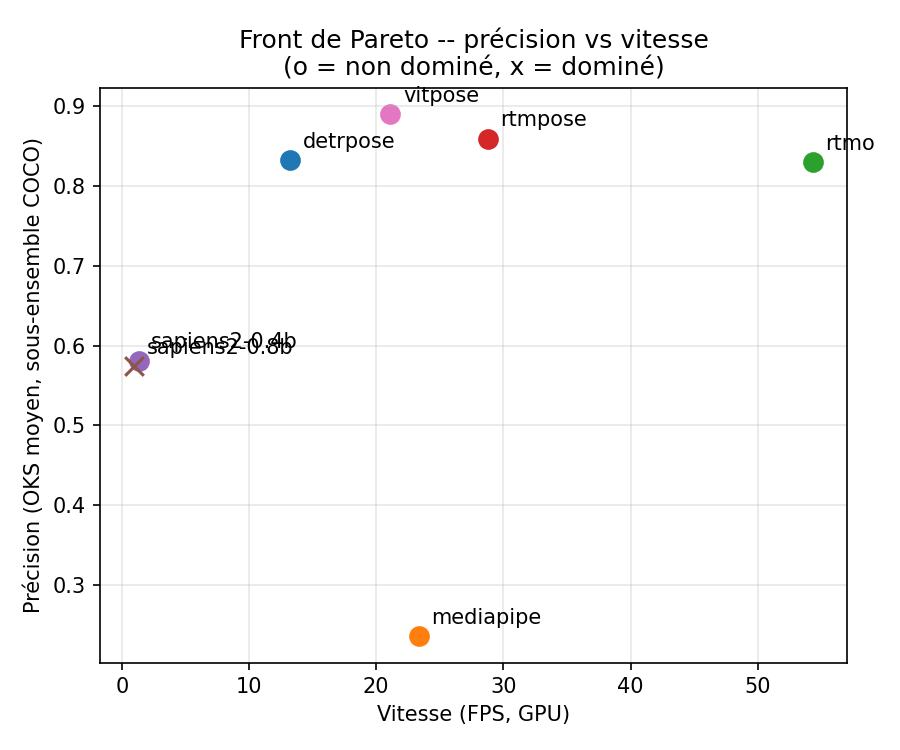
\includegraphics[width=0.85\textwidth]{../benchmark/results/pareto.png}}{\fbox{pareto.png introuvable}}
\caption{Front de Pareto précision/vitesse du banc de recherche (\code{research/benchmark/results/pareto.png}).}
\label{fig:pareto}
\end{figure}

Dans ce banc, ViTPose reçoit les boîtes de la vérité terrain COCO (évaluation \enquote{boîtes oracle}, qui isole
la qualité de la pose de celle de la détection), et celles du détecteur de RTMPose sur la vidéo.

\section{Intégration dans psifx}
\label{sec:res-integration}

\begin{table}[H]
\centering
\caption{Modèles intégrés, mesurés via la commande psifx (vidéo de 50 images COCO, et extrait de test de 8 images).
Ici, ViTPose utilise un vrai détecteur (RT-DETR) et non les boîtes de la vérité terrain.}
\label{tab:integration}
\begin{tabular}{@{}lccccc@{}}
\toprule
& \multicolumn{3}{c}{50 images} & \multicolumn{2}{c}{8 images (test)} \\
\cmidrule(lr){2-4}\cmidrule(lr){5-6}
Commande psifx & OKS & PCK & Détection & OKS & PCK \\
\midrule
\code{mediapipe} (actuel) & 0,283 & 0,432 & 84\,\% & 0,647 & 0,968 \\
\code{rtmpose} & \textbf{0,873} & \textbf{0,935} & 98\,\% & 0,935 & 0,988 \\
\code{vitpose} & 0,850 & 0,914 & 96\,\% & 0,943 & 0,988 \\
\code{detrpose} & 0,840 & 0,922 & 98\,\% & \textbf{0,951} & \textbf{1,000} \\
\code{rtmo} & 0,826 & 0,880 & 92\,\% & 0,943 & \textbf{1,000} \\
\bottomrule
\end{tabular}
\end{table}

Les quatre intégrations reproduisent les niveaux du banc de recherche (écarts de 0,01 à 0,04 d'OKS, expliqués par
le passage en vidéo, la sélection d'une seule personne et, pour ViTPose, le passage des boîtes oracle à un vrai
détecteur). Tous gagnent plus de 0,5 d'OKS sur MediaPipe.

\section{Optimisations d'inférence}
\label{sec:res-optim}

\begin{table}[H]
\centering
\caption{Vitesse en régime établi (50 images COCO) et précision via la commande psifx, par modèle et par
optimisation. Gain relatif à fp32 sur le même appareil. Pour DETRPose : temps du modèle seul.}
\label{tab:optim}
\small
\begin{tabular}{@{}lllrrcc@{}}
\toprule
Modèle & Appareil & Configuration & ms/image & Gain & OKS & Détection \\
\midrule
\multirow{5}{*}{RTMPose} & CPU & fp32 & 274,5 & -- & 0,873 & 98\,\% \\
& CPU & int8 & 436,9 & $-59$\,\% & 0,647 & 98\,\% \\
& GPU & fp32 & 24,6 & -- & 0,873 & 98\,\% \\
& GPU & fp16 & 22,1 & $+11$\,\% & 0,873 & 98\,\% \\
& GPU & int8 & 32,3 & $-31$\,\% & 0,648 & 96\,\% \\
\midrule
\multirow{5}{*}{RTMO} & CPU & fp32 & 149,1 & -- & 0,826 & 92\,\% \\
& CPU & int8 & 255,6 & $-42$\,\% & 0,584 & 72\,\% \\
& GPU & fp32 & 13,0 & -- & 0,826 & 92\,\% \\
& GPU & \textbf{fp16} & \textbf{9,1} & $\mathbf{+43}$\,\% & 0,826 & 92\,\% \\
& GPU & int8 & 17,7 & $-26$\,\% & 0,580 & 70\,\% \\
\midrule
\multirow{4}{*}{ViTPose} & GPU & fp32 & 55,1 & -- & 0,850 & 96\,\% \\
& GPU & fp16 & 56,9 & $-3$\,\% & 0,850 & 96\,\% \\
& GPU & compile & 64,5 & $-17$\,\% & -- & -- \\
& GPU & fp16 + compile & 50,0 & $+10$\,\% & 0,851 & 96\,\% \\
\midrule
\multirow{5}{*}{DETRPose} & CPU & fp32 & 297,9 & -- & 0,840 & 98\,\% \\
& GPU & fp32 & 23,9 & -- & 0,840 & 98\,\% \\
& GPU & fp16 & 35,8 & $-33$\,\% & 0,840 & 98\,\% \\
& GPU & compile & 15,4 & $+55$\,\% & 0,839 & 98\,\% \\
& GPU & fp16 + compile & 11,9 & $\times 2{,}0$ & 0,840 & 98\,\% \\
\bottomrule
\end{tabular}
\end{table}

\subsection{Où part le temps}

\begin{table}[H]
\centering
\begin{minipage}[t]{0.48\textwidth}
\centering
\caption{ViTPose fp32 : temps par étape (ms/image).}
\label{tab:vitpose-profil}
\small
\begin{tabular}{@{}lrr@{}}
\toprule
Étape & ms & Part \\
\midrule
Prétrait. détecteur (CPU) & 2,7 & 5\,\% \\
\textbf{Détecteur RT-DETR} & \textbf{26,7} & \textbf{45\,\%} \\
Post-trait. détecteur & 0,5 & 1\,\% \\
\textbf{Prétrait. ViTPose (CPU)} & \textbf{12,8} & \textbf{22\,\%} \\
Modèle ViTPose & 13,5 & 23\,\% \\
Post-trait. ViTPose & 3,1 & 5\,\% \\
\bottomrule
\end{tabular}
\end{minipage}
\hfill
\begin{minipage}[t]{0.48\textwidth}
\centering
\caption{DETRPose, GPU : coût fixe et coût par image, de bout en bout.}
\label{tab:detrpose-pont}
\small
\begin{tabular}{@{}lrrr@{}}
\toprule
Config. & Fixe & ms/img & Modèle \\
\midrule
fp32 & 2,6\,s & 90,1 & 21,7 \\
fp16 + compile & 8,2\,s & 101,6 & 14,4 \\
\bottomrule
\end{tabular}
\end{minipage}
\end{table}

Pour ViTPose, le transformeur ciblé par l'optimisation ne représente qu'environ 23\,\% du temps : même un gain
parfait sur lui plafonnerait à environ 1,3$\times$ de bout en bout. Pour DETRPose, environ 70\,ms par image partent
dans le pont entre psifx et l'environnement de DETRPose (écriture et relecture PNG, prétraitement PIL) : l'effet
de l'optimisation du modèle disparaît presque entièrement de bout en bout.

% =============================================================================
\chapter{Discussion}
\label{chap:discussion}
% =============================================================================

\section{Réponses aux questions}

\paragraph{Q1 -- Gain de précision.} Il est massif : de 0,235 (MediaPipe) à 0,830--0,890 d'OKS dans le banc de
recherche, et de 0,283 à 0,826--0,873 via la commande psifx. Nos propres mesures confirment ainsi les comparatifs
indépendants \cite{circus2026mediapipe,gait2022comparison}. Sapiens2, pourtant le plus récent, perd 25 à 30 points
face aux meilleurs candidats dans nos conditions (détecteur par défaut, bf16), et toutes ses tailles restent sous
1,5 image/s.

\paragraph{Q2 -- Stabilité temporelle.} Précision et stabilité sont largement indépendantes, comme le suggère le
cadre MBRCS \cite{fernandez2026mbrcs}. MediaPipe est le plus stable mais le moins précis : il lisse ses
prédictions dans le temps, alors que les autres modèles traitent chaque image indépendamment. RTMPose est le plus
précis des modèles rapides mais le moins stable. RTMO et DETRPose se situent entre les deux. Le jerk ne fait donc
pas qu'opposer des modèles : il compare aussi des modèles avec et sans lissage temporel.

\paragraph{Q3 -- Vitesse et mémoire.} Sur GPU, RTMO est de loin le plus rapide (13\,ms/image en fp32, 9,1\,ms en
fp16 via psifx). Sur CPU, tous les candidats restent utilisables pour du traitement différé (150 à 300\,ms/image),
avec un facteur d'environ 11 en faveur du GPU, bien plus que n'importe quelle optimisation de modèle.

\paragraph{Q4 -- Dominance.} Aucun modèle ne domine sur toutes les dimensions : six configurations sur sept sont
sur le front de Pareto. Le choix se resserre à deux candidats :
\begin{itemize}
    \item \textbf{ViTPose} (ou RTMPose, très proche via psifx) si la précision prime ;
    \item \textbf{RTMO} pour le compromis précision/vitesse/simplicité : un seul modèle, pas de détecteur à
    maintenir, premier du classement pondéré, et le seul à profiter pleinement du fp16.
\end{itemize}
Tous deux sont sous Apache 2.0. Plutôt que de trancher entre traitement différé (précision) et pipeline proche du
temps réel (vitesse), les deux ont été intégrés : l'utilisateur choisit selon son étude
(section~\ref{sec:decisions}).

\paragraph{Q5 -- Optimisations.} Le fp16 est un gain gratuit sur GPU pour les modèles ONNX (+11\,\% RTMPose,
+43\,\% RTMO), sans aucune perte de précision. \code{torch.compile} combiné au fp16 double la vitesse du modèle
DETRPose et gagne 10\,\% sur ViTPose, mais coûte de 8\,s à 2\,min de compilation à chaque appel de la commande, et
son effet est masqué par les étapes hors modèle. L'INT8 statique est à écarter sur ce matériel : plus lent sur CPU
comme sur GPU, et 23 à 24 points d'OKS en moins.

\section{Décisions d'intégration}
\label{sec:decisions}

Sur la base de ces résultats, les choix suivants ont été faits pour la branche principale de psifx
(tableau~\ref{tab:decisions}) :
\begin{itemize}
    \item \textbf{RTMO}, avec l'option \code{--precision fp16}, et \textbf{ViTPose} rejoignent la bibliothèque. RTMO
    offre le meilleur compromis et le seul gain fp16 notable ; ViTPose est le plus précis des modèles retenus et
    n'ajoute aucune dépendance.
    \item \textbf{RTMPose} et \textbf{DETRPose} restent dans leurs branches : RTMPose fait en grande partie doublon
    avec RTMO (même dépendance) et ViTPose ; DETRPose demande un environnement séparé et souffre d'un pont lent.
    \item L'\textbf{INT8} et les options fp16 et \code{torch.compile} de ViTPose sont retirés : défavorables ou
    marginaux pour un coût réel.
    \item \code{rtmlib} devient une dépendance optionnelle (\code{psifx[rtm]}, \code{psifx[rtm-gpu]}) : l'installation
    de base de psifx est inchangée. Les paquets \code{onnxruntime} et \code{onnxruntime-gpu} s'installent dans le
    même dossier et s'écrasent mutuellement ; la documentation indique comment ne garder que la version GPU, et
    l'outil charge lui-même cuDNN et cuBLAS installés avec PyTorch.
    \item Le matériel de recherche (notes, banc de mesure, rapport) reste hors de la bibliothèque ; le code
    d'évaluation COCO utilisé par les tests a été déplacé dans \code{tests/pose_eval/}.
\end{itemize}

\begin{table}[H]
\centering
\caption{Récapitulatif des modèles et optimisations, et décision pour la bibliothèque (50 images COCO, GPU sauf
mention ; temps en régime établi ; DETRPose : modèle seul).}
\label{tab:decisions}
\footnotesize
\begin{tabular}{@{}llrccl@{}}
\toprule
Modèle & Configuration & ms/image & OKS & Détection & Décision \\
\midrule
MediaPipe & -- (CPU) & -- & 0,283 & 84\,\% & conservé (visage, mains) \\
\textbf{RTMO} & fp32 / \textbf{fp16} & 13,0 / \textbf{9,1} & 0,826 & 92\,\% & \textbf{bibliothèque} \\
\textbf{ViTPose} & fp32 & 55,1 & 0,850 & 96\,\% & \textbf{bibliothèque} \\
RTMPose & fp32 / fp16 & 24,6 / 22,1 & 0,873 & 98\,\% & branche \\
DETRPose & fp32 / fp16 + compile & 23,9 / 11,9 & 0,840 & 98\,\% & branche \\
Tous ONNX & int8 & plus lent & 0,58--0,65 & 70--98\,\% & retiré \\
ViTPose & fp16 + compile & 50,0 & 0,851 & 96\,\% & retiré \\
\bottomrule
\end{tabular}
\end{table}

\section{Pourquoi l'INT8 échoue ici}

Trois causes, cohérentes avec la documentation d'ONNX Runtime \cite{ort_quantization} :
\begin{enumerate}
    \item dans les modèles OpenMMLab, l'activation SiLU (\code{Sigmoid} $\times$ \code{Mul}) reste en float entre
    chaque convolution, ce qui impose une paire Quantize/Dequantize à chaque couche et annule le gain des
    convolutions INT8, même sur un CPU doté d'AVX-VNNI ;
    \item le provider CUDA n'a pas de vrais noyaux INT8 pour ce format ; il faudrait TensorRT et les Tensor Cores INT8
    \cite{ort_tensorrt} ;
    \item la perte de précision vient des convolutions elles-mêmes : ne quantifier que les \code{Conv} donne le
    même OKS (0,657 contre 0,647 pour RTMPose).
\end{enumerate}

\section{Enseignements méthodologiques}

Plusieurs écueils rencontrés valent d'être notés, car ils faussent silencieusement des mesures :
\begin{itemize}
    \item \textbf{Chronométrer sans synchronisation CUDA} : l'exécution GPU est asynchrone, le temps mesuré
    n'inclut alors que le lancement des noyaux \cite{pytorch_cuda_async}. Le script DETRPose du banc de recherche
    avait ce défaut ; le chiffre de 13,3\,FPS du tableau~\ref{tab:banc} est donc à remesurer.
    \item \textbf{Retombée silencieuse sur CPU} : sans cuDNN sur le \code{LD_LIBRARY_PATH}, \code{onnxruntime-gpu}
    s'exécute sur CPU sans erreur bloquante. Les outils psifx lèvent désormais une erreur explicite.
    \item \textbf{Quantification naïve} : quantifier tous les opérateurs a donné un OKS nul. La sortie du détecteur
    YOLOX concatène coordonnées (0 à 640) et scores (0 à 1), et une seule échelle INT8 ramène tous les scores à 0.
    Un test de non-régression couvre désormais ce cas.
    \item \textbf{Conflits de dépendances} : installer \code{onnx} 1.23 fait passer protobuf en version 7 et casse
    MediaPipe ; installer les dépendances de DETRPose dans l'environnement de psifx casse numpy, scipy et OpenCV.
    D'où les environnements séparés et les versions épinglées.
    \item \textbf{Contention GPU} : un GPU partagé fausse les vitesses absolues ; seules les comparaisons au sein
    d'une même passe sont fiables.
    \item \textbf{Profiler avant d'optimiser} : la cible annoncée de l'optimisation (le transformeur pour ViTPose,
    le modèle pour DETRPose) n'était pas le goulot.
\end{itemize}

\section{Limites}

\begin{itemize}
    \item Échantillons réduits (50 et 8 images COCO, une seule personne annotée par image) : les comparaisons
    relatives sont valides, pas les valeurs absolues face à val2017 complet. Le sous-comptage de DETRPose sur les
    scènes très peuplées (1 personne trouvée sur 26 au seuil 0,5) n'est pas capturé par ce protocole.
    \item Une seule vidéo pour la stabilité, sans vérité terrain ; le jerk est biaisé par le lissage de MediaPipe.
    \item L'occlusion mutuelle, cas réel de psifx, n'est pas évaluée spécifiquement (CrowdPose non utilisé).
    \item Les intégrations ne suivent qu'une personne par vidéo, comme MediaPipe ; le multi-personnes passe par les
    masques SAM3.
    \item Licence de Sapiens2 non validée ; Sapiens2-1B non re-mesuré dans la dernière passe.
\end{itemize}

% =============================================================================
\chapter{Approfondissements et test de bout en bout}
\label{chap:phase2}
% =============================================================================

Ce chapitre couvre la phase qui a suivi la réunion de suivi du 13 octobre 2026 : les quatre demandes faites à cette
réunion, puis un test de bout en bout de psifx sur des vidéos réelles, et la correction du suivi SAM3 que ce test a
rendue nécessaire. Il se termine par une veille des solutions apparues depuis le début du travail.

\section{Suites de la réunion du 13 octobre}
\label{sec:phase2-reunion}

\subsection{Pourquoi ViTPose est moins bon que prévu}

Dans psifx, ViTPose-B obtient 0,850 d'OKS, sous RTMPose-m (0,873), alors que le banc de recherche lui donnait 0,890.
L'analyse (branche \code{analysis/vitpose-gap}) mesure chaque facteur séparément (tableau~\ref{tab:vitpose-gap}),
avec des intervalles de confiance à 95\,\% par bootstrap apparié.
\begin{itemize}
    \item \textbf{La littérature ne prédit pas d'avantage net à taille égale} : 75,5 AP pour ViTPose-B (COCO seul)
    contre 74,9 pour RTMPose-m \cite{xu2022vitpose,jiang2023rtmpose}. La réputation de ViTPose vient de ses grandes
    variantes.
    \item \textbf{Le banc de recherche n'était pas à armes égales} : ViTPose y recevait les boîtes de la vérité
    terrain. À boîtes égales, les deux modèles sont à égalité.
    \item \textbf{L'écart observé dans psifx n'est pas significatif} sur 50 images (différence $-0{,}022$, IC
    $[-0{,}066\,;\,+0{,}008]$). Le détecteur coûte environ 0,036 d'OKS à ViTPose.
    \item \textbf{Leviers} : une variante plus grande (ViTPose++ L, +0,02 avec boîtes parfaites), le \emph{flip test}
    (+0,006, faible mais significatif) et un meilleur choix de la personne suivie.
\end{itemize}

\begin{table}[H]
\centering
\caption{OKS moyen sur 50 images COCO selon la source des boîtes.}
\label{tab:vitpose-gap}
\small
\begin{tabular}{@{}lcc@{}}
\toprule
Boîtes & ViTPose-B & RTMPose-m \\
\midrule
Vérité terrain (pose seule) & 0,889 & 0,896 \\
YOLOX, bonne personne & 0,849 & 0,858 \\
RT-DETR, bonne personne & 0,862 & 0,859 \\
Réglage psifx (vidéo, détecteur propre, plus grande boîte) & 0,850 & 0,873 \\
\bottomrule
\end{tabular}
\end{table}

\subsection{Cause de l'échec de l'INT8}

L'analyse (branche \code{analysis/int8-root-cause}, RTMPose sur CPU) explique les deux symptômes de la
section~\ref{sec:res-optim}.
\begin{itemize}
    \item \textbf{Précision} : toute la perte vient du modèle de pose. Le détecteur quantifié seul garde son OKS
    (0,856 contre 0,858), le modèle de pose seul tombe à 0,664. Ce n'est pas la calibration : trois méthodes donnent
    le même résultat, et calibrer sur les images évaluées fait même pire. Le rapport signal/bruit des activations
    reste vers 21\,dB dans la première moitié du réseau, puis tombe à 2,7\,dB aux trois quarts : l'erreur est
    répartie et cumulative, et la tête SimCC, qui demande une résolution fine, ne la supporte pas. Garder en float
    les 20 couches les plus sensibles ne remonte qu'à 0,690.
    \item \textbf{Vitesse} : 57 des 62 convolutions alimentent une activation SiLU qui lit leur sortie deux fois.
    ONNX Runtime ne forme alors jamais le motif qu'il remplace par une convolution entière : seules 4 convolutions
    deviennent \code{QLinearConv}, les autres restent en float, entourées de 450 conversions. Le modèle de pose passe
    de 13,6 à 34,2\,ms.
    \item \textbf{Conséquence} : la décision de retirer l'INT8 est confirmée. Seuls un ré-entraînement avec
    quantification simulée (QAT) ou un moteur qui fusionne Conv et SiLU en INT8 (TensorRT) pourraient changer ce
    constat \cite{ort_quantization,ort_tensorrt}.
\end{itemize}

\subsection{Une seule commande pour RTMO et ViTPose}

\code{psifx video pose body} (branche \code{feature/pose-body-command}) regroupe les deux modèles retenus :
RTMO par défaut, ViTPose avec \code{--model vitpose}. Les deux outils sous-jacents restent inchangés ; la commande
ne fait que choisir l'un ou l'autre, avec les mêmes sorties que \code{mediapipe}, y compris en multi-personnes
(\code{multi-inference} sur les masques SAM3).

\subsection{Test de précision sur un jeu complet : OCHuman}

Les 8 images COCO du test de non-régression sont connues des modèles et trop peu nombreuses : des écarts de 0,01 à
0,02 y sont du bruit. Un test d'intégration sur toute la partie test d'OCHuman \cite{zhang2019pose2seg} (2231
images de personnes occultées, branche \code{feature/tests-ochuman}) le complète. Il calcule l'AP COCO avec
\code{pycocotools} et ne tourne qu'à la demande (marqueur \code{dataset}, variable \code{OCHUMAN_ROOT}).
\begin{itemize}
    \item AP mesurés : RTMO-m 0,289, ViTPose-B 0,343. Seuils du test fixés environ 3 points en dessous (0,26 et
    0,31).
    \item Ces AP sont bas par construction : OCHuman n'annote pas toutes les personnes, donc une détection correcte
    d'une personne non annotée compte comme faux positif ; et les personnes très occultées échappent souvent aux
    détecteurs. Le test sert à détecter une régression, pas à situer les modèles dans la littérature.
\end{itemize}

\section{Test de bout en bout}
\label{sec:e2e}

\subsection{Objectif et chaîne testée}

Les chapitres précédents mesurent la pose sur des images. Ce test vérifie que psifx transforme des vidéos réelles
et variées en données exploitables, puis le montre par un usage concret : reconstruire une vidéo où chaque personne
est un squelette 2D d'une couleur fixe, avec un panneau 3D simple et des sous-titres de la couleur de la personne
qui parle. Les scripts sont dans \nolinkurl{research/e2e/} (branche \code{experiment/e2e-demo}). Chaque étape est une
commande psifx ou un script de recherche, chronométrée, et la chaîne s'arrête à la première erreur
(tableau~\ref{tab:e2e-chaine}).

\begin{table}[H]
\centering
\caption{Chaîne de bout en bout.}
\label{tab:e2e-chaine}
\small
\begin{tabularx}{\textwidth}{@{}lY@{}}
\toprule
Étape & Outil \\
\midrule
Suivi des personnes & \code{psifx video tracking sam3 inference} (un masque par personne) \\
Poses & \code{psifx video pose body} (RTMO), \code{psifx video pose mediapipe} (visage, mains, et nouvelle clé
\code{pose_keypoints_3d} : points 3D du corps en mètres) \\
Audio & extraction, conversion, normalisation psifx ; séparation de la voix par Demucs \cite{rouard2023htdemucs} pour la musique \\
Qui parle quand & \code{psifx audio diarization pyannote} (\code{speaker-diarization-3.1} \cite{pyannote31}) \\
Transcription & \code{psifx audio transcription whisperx} (\code{large-v3-turbo}, multilingue) \cite{bain2023whisperx} \\
Voix $\leftrightarrow$ personne & script de recherche : mouvement des lèvres (MediaPipe) et présence à l'écran,
corrélés aux tours de parole ; affectation hongroise, sinon \enquote{hors champ} \\
Sous-titres attribués & \code{psifx audio transcription enhance}, avec l'association précédente \\
Re-rendu et mesures & scripts de recherche : vidéo avec squelettes, panneau 3D et sous-titres colorés, fichier
\code{.ass}, métriques \\
\bottomrule
\end{tabularx}
\end{table}

psifx ne relie une voix à une personne visible que si chacune porte un micro (\code{audio identification}). Le
script d'association par les lèvres comble ce manque sans matériel : il sort le même format, donc
\code{transcription enhance} l'utilise sans changement.

\subsection{Vidéos}

\begin{table}[H]
\centering
\caption{Vidéos du test, de la plus simple à la plus difficile.}
\label{tab:e2e-videos}
\small
\begin{tabularx}{\textwidth}{@{}lrYY@{}}
\toprule
Vidéo & Durée & Difficulté & Vérité terrain \\
\midrule
V1 \code{Video.mp4} (exemple psifx) & 46\,s & 1 personne visible, 1 voix hors champ & 1 micro par personne (stéréo) \\
V2 AVA-ActiveSpeaker \cite{roth2020ava} & 2\,min & 2 personnes, espagnol, plan fixe & visages annotés \enquote{parle / ne parle pas} \\
V3 talk-show (Konbini) & 5,5\,min & français, 2 personnes, 112 changements de plan, incrustations & aucune \\
V4 \emph{short} de danse & 48\,s & personnage animé avec une queue, mouvements rapides, voix sous la musique & paroles (WER) \\
\bottomrule
\end{tabularx}
\end{table}

Le corpus AMI, prévu au départ pour les réunions, n'a pas pu être utilisé : son site refuse les connexions et ses
copies vidéo sur Hugging Face ont disparu. AVA-ActiveSpeaker le remplace pour mesurer l'association voix--personne.

\subsection{Résultats}

\begin{table}[H]
\centering
\caption{Résultats par vidéo. Facteur temps réel : temps de calcul total divisé par la durée de la vidéo.}
\label{tab:e2e-resultats}
\small
\begin{tabular}{@{}lcccccc@{}}
\toprule
& & \multicolumn{2}{c}{Poses trouvées} & Voix & Texte sur une & Facteur \\
\cmidrule(lr){3-4}
Vidéo & Pistes & RTMO & MediaPipe & diarisées & personne visible & temps réel \\
\midrule
V1 & 1 & 100\,\% & 100\,\% & 2 & 49\,\% & 21,3$\times$ \\
V2 & 2 & 97--100\,\% & 100\,\% & 4 & 76\,\% & 24,5$\times$ \\
V3 & 3 (sur 18) & 63--70\,\%$^*$ & 63--71\,\%$^*$ & 3 & 100\,\% & 27,8$\times$ \\
V4 & 1 & 87\,\% & 94\,\% & 1 & 0\,\% & 18,3$\times$ \\
\bottomrule
\end{tabular}

\smallskip
\footnotesize $^*$ Part de toutes les images ; à cause du montage, les deux personnes ne sont à l'écran que sur 64 et
72\,\% des images, et une pose est trouvée sur 98\,\% des images où elles le sont.
\end{table}

\begin{itemize}
    \item \textbf{Association voix--personne}. V1 : 100\,\% d'accord avec les micros ; la voix hors champ est bien
    classée hors champ. V2 : sur 1784 instants où quelqu'un parle, la personne désignée est la bonne dans 65\,\% des
    cas, contre 52\,\% par hasard. L'association ne répond que pour 72\,\% de ces instants, mais a raison à 90\,\%
    quand elle répond. Les non-réponses viennent de la diarisation, qui trouve 4 voix pour 2 personnes.
    V3 : sans vérité terrain, 40 segments de transcription ont été étiquetés d'après le texte seul quand il ne laisse
    aucun doute (questions de l'intervieweur, invitée parlant d'elle au féminin). Avec les lèvres seules, 59\,\% du
    temps de ces segments était attribué à la bonne personne : la voix de l'intervieweur partait \enquote{hors
    champ}, car ses lèvres, derrière une barbe et un micro, bougent à peine plus quand il parle. Un second terme
    corrige ce cas : dans une vidéo montée, la réalisation montre le plus souvent la personne qui parle. Le score
    ajoute donc la part du temps de parole où la personne est à l'écran, moins cette part pendant que les autres
    parlent. Ce terme est nul pour une caméra fixe où tout le monde reste visible : V1, V2 et V4 sont inchangés, et V3
    passe à 98\,\% (39 segments sur 40). Le lien de l'intervieweur reste juste au-dessus du seuil (score 0,26 pour
    un seuil de 0,2).
    \item \textbf{Transcription sous la musique (V4)}. Sans séparation de la voix, WhisperX ne détecte aucune parole et
    plante. Avec Demucs, le WER vaut 0,58 ; une seule expression du refrain mal entendue en coûte environ 15 points.
    \item \textbf{Coût}. Le suivi SAM3 domine (13 à 19$\times$ le temps réel sur la RTX 4060, davantage quand la
    vidéo est montée), devant MediaPipe sur CPU (2 à 5$\times$). Une heure de vidéo demanderait de 13 à 19\,h de suivi
    sur ce portable.
\end{itemize}

\begin{figure}[H]
\centering
\IfFileExists{figures/e2e_v3_frame.jpg}{%
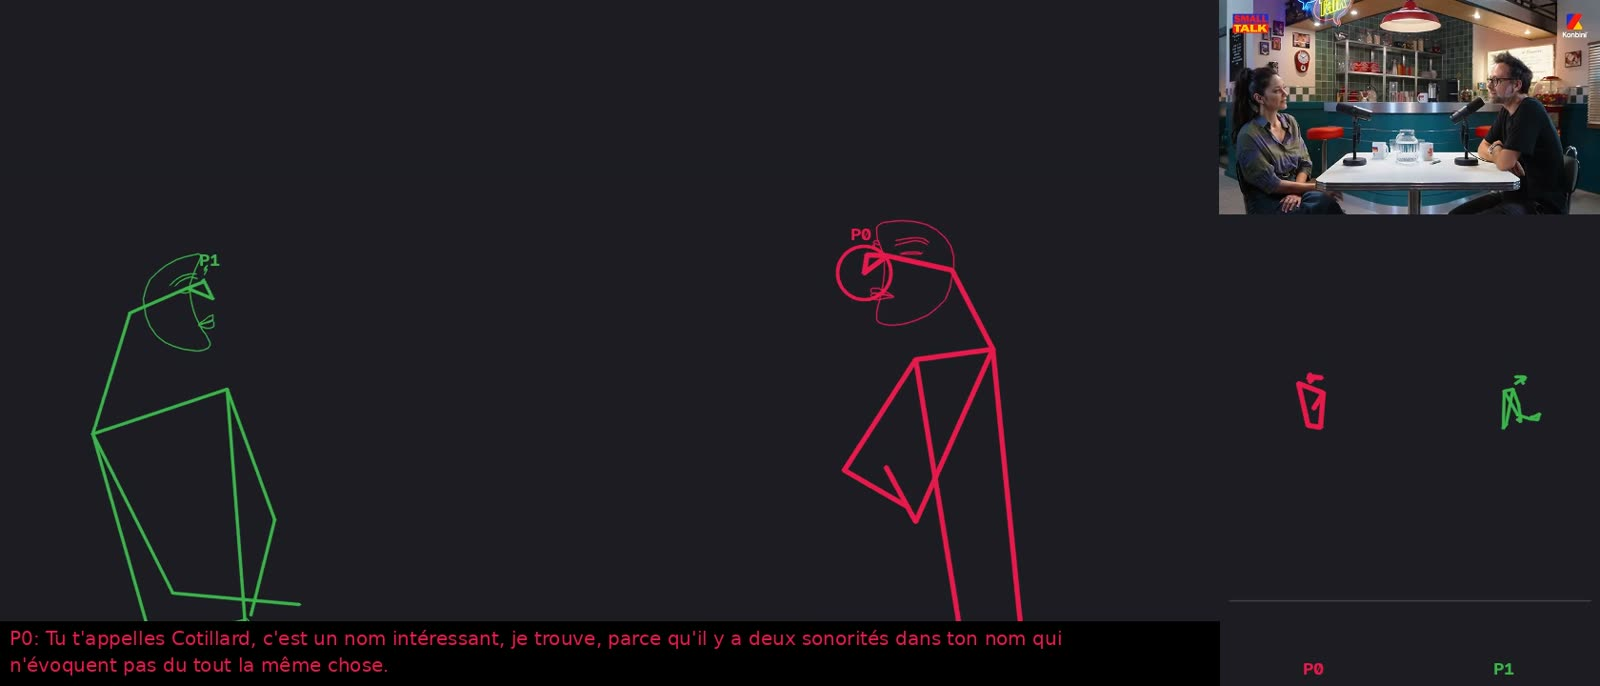
\includegraphics[width=\textwidth]{figures/e2e_v3_frame.jpg}}{\fbox{e2e\_v3\_frame.jpg introuvable}}
\caption{Image de la vidéo reconstruite pour V3 : squelettes 2D d'une couleur par personne, vignette de l'original
et panneau 3D à droite, sous-titre de la couleur de la personne qui parle.}
\label{fig:e2e-v3}
\end{figure}

\subsection{Limites observées}

\begin{itemize}
    \item \textbf{Visage non humain} (V4) : MediaPipe ne trouve le visage animé que sur 7\,\% du temps chanté ; sans
    lèvres, pas d'association. Le corps est bien suivi, la queue est ignorée (absente des squelettes).
    \item \textbf{Sur-découpage de la diarisation} : plusieurs voix pour une même personne, que l'association rattache
    quand le score le permet.
    \item \textbf{Granularité de \code{enhance}} : chaque segment de transcription reçoit un seul locuteur ; une
    réplique rapide à l'intérieur d'un segment prend la couleur de l'autre personne.
    \item \textbf{Montage} (V3) : le suivi SAM3 ne supportait pas les changements de plan
    (section~\ref{sec:sam3-plans}). Le filtre de présence garde aussi une piste qui n'est pas une personne : une
    main en très gros plan, dans un plan qui revient sur 15\,\% de la vidéo.
    \item \textbf{Lèvres peu lisibles} (V3) : barbe et micro devant la bouche ; compensé ici par la présence à
    l'écran, qui ne servirait à rien sur un plan fixe.
\end{itemize}

Le test a aussi révélé quatre défauts de psifx, contournés dans les scripts : le modèle d'identification par défaut
(speechbrain) ne se charge plus avec un \code{huggingface_hub} récent ; WhisperX plante au lieu de rendre une
transcription vide quand il ne détecte aucune parole ; l'option \code{--language} de la transcription n'est jamais
transmise ; MediaPipe écrit 468 points de visage quand il n'en trouve pas, mais 478 sinon.

\section{Suivi SAM3 à travers les changements de plan}
\label{sec:sam3-plans}

\subsection{Le problème}

Sur le talk-show, le suivi a atteint 57 pistes pour 2 personnes, puis a saturé la mémoire de l'ordinateur. Deux
mécanismes sont en cause.
\begin{itemize}
    \item \textbf{Identités perdues ou échangées au changement de plan}. psifx découpe la vidéo en paquets et relie les
    identités d'un paquet au suivant par le recouvrement des masques. Après une coupe, les masques ne se recouvrent
    plus : chaque personne reçoit un nouvel identifiant. Pire, quand deux gros plans alternent au même endroit de
    l'image, la mémoire de SAM3 et le recouvrement font passer l'identité d'une personne à l'autre. Sur la première
    minute, 16 pistes, dont 4 mélangent les deux personnes.
    \item \textbf{Un encodeur vidéo par piste}. Chaque piste garde un encodeur x264 ouvert jusqu'à la fin, en 1080p et
    sans perte : environ 800\,Mo de RAM chacun, 43\,Go pour les 58 pistes.
\end{itemize}
La littérature confirme que SAM2 et SAM3 perdent les objets aux changements de scène et que leur mémoire ne règle pas
les ambiguïtés d'identité \cite{pvuw2026reprompt}. Les travaux sur les séries télévisées découpent la vidéo en plans
et relient ensuite les personnes d'un plan à l'autre par l'apparence ou la géométrie
\cite{pavlakos2022tvshows,multithumbs2026}.

\subsection{La correction}

La correction (branche \code{fix/sam3-shot-changes}, mergée dans \code{dev}) suit ce schéma.
\begin{enumerate}
    \item \textbf{Détection des coupes} : différence moyenne entre deux vignettes consécutives de 64$\times$36 pixels,
    au-dessus de 0,15 et nettement au-dessus du mouvement récent. Sur la première minute du talk-show, elle retrouve
    les 30 coupes détectées par \code{ffmpeg}, plus 3 animations, et ne déclenche aucune fausse coupe sur V1, V2 et
    la danse.
    \item \textbf{Une session SAM3 par plan} : aucune identité n'est transmise à travers une coupe.
    \item \textbf{Ré-identification par l'apparence} : chaque nouvelle piste reçoit l'identifiant de la personne la plus
    semblable déjà vue, si la similarité cosinus dépasse 0,45, sinon un nouvel identifiant. L'apparence est un
    plongement DINOv2-small \cite{oquab2023dinov2} de la personne découpée par son masque, fond grisé. Deux pistes
    visibles dans la même image ne peuvent pas recevoir le même identifiant. Avec \code{--max_num_objects}, une fois
    la limite atteinte, la nouvelle piste prend l'identifiant le plus proche au lieu d'être abandonnée.
    \item \textbf{Mémoire} : les encodeurs passent en \code{-tune zerolatency}, qui supprime le tampon d'anticipation
    de x264 \cite{x264_memory} : 813 à 170\,Mo par encodeur, toujours sans perte.
    \item \textbf{Post-traitement de SAM3} : sans le paquet optionnel \code{kernels}, \code{transformers} saute la
    suppression des détections en double (NMS) et le remplissage des trous des masques \cite{hf_kernels}. Ce paquet
    télécharge du code compilé depuis le Hub à l'exécution ; psifx fournit donc ses propres versions de ces deux
    opérations, en PyTorch et SciPy.
\end{enumerate}

\subsection{Mesures}

Le descripteur d'apparence a été choisi sur 41 segments (une piste dans un plan) étiquetés à la main. DINOv2 sépare
bien mieux les deux personnes qu'un histogramme de couleurs (tableau~\ref{tab:reid}), ce qui rejoint les études
récentes sur la ré-identification sans entraînement spécifique \cite{reid2026survey}. Simulée en ligne, dans l'ordre
du temps, l'attribution regroupe les 41 segments en 5 identités sans aucune erreur : les 2 personnes, et 3
identités pour les incrustations graphiques.

\begin{table}[H]
\centering
\caption{Choix du descripteur : 41 segments de la première minute de V3. AUC : probabilité qu'une paire de la même
personne soit plus semblable qu'une paire de personnes différentes.}
\label{tab:reid}
\small
\begin{tabular}{@{}lcc@{}}
\toprule
Descripteur & AUC & Meilleure exactitude par paire \\
\midrule
Histogramme teinte--saturation des pixels du masque & 0,708 & 0,710 \\
DINOv2-small (classe, moyenne de 8 vues) & \textbf{0,966} & \textbf{0,913} \\
\bottomrule
\end{tabular}
\end{table}

\begin{table}[H]
\centering
\caption{Suivi SAM3 sur la première minute de V3 (1502 images, 2 personnes, 30 coupes).}
\label{tab:sam3-plans}
\small
\begin{tabular}{@{}lccc@{}}
\toprule
Version & Pistes & Pistes mélangeant les 2 personnes & Temps \\
\midrule
Avant & 16 & 4 & 1143\,s \\
NMS seule & 16 & -- & 1162\,s \\
\textbf{Coupes + ré-identification + NMS} & \textbf{9} & \textbf{0} & \textbf{1032\,s} \\
\bottomrule
\end{tabular}
\end{table}

Avec la correction, chaque personne tient en une seule piste continue sur les 33 plans. Les 7 autres pistes sont des
incrustations (logo, photo de l'invitée dans le générique), une main en très gros plan et des fragments de quelques
images ; le pipeline de bout en bout les écarte avant l'estimation de pose s'ils sont présents sur moins de 5\,\% de
la vidéo. La NMS seule ne change pas le nombre de pistes : le problème venait bien des coupes. Sur V1, sans coupe,
le résultat ne change pas (1 piste, IoU moyenne de 0,974 avec les anciens masques, différences dues au remplissage
des trous), pour 7\,\% de temps en plus.

Sur la vidéo complète de V3 (8319 images, 113 plans détectés), le suivi donne 18 pistes, contre plus de 57 à 76\,\%
de la vidéo avant la correction, et la mémoire reste stable. Chacune des deux personnes tient en une seule piste
pure sur les 5,5 minutes. Les 15 autres pistes sont présentes sur moins de 2,5\,\% des images, sauf la main en gros
plan (15\,\%). Le suivi prend 6192\,s, soit 18,6$\times$ le temps réel.

\section{Diarisation : pyannote \code{community-1}}
\label{sec:community1}

pyannote a publié en 2025 le pipeline \code{community-1} \cite{pyannote_community1}, qui demande
\code{pyannote.audio}~4. Il a été comparé à la \code{3.1} sur sa propre branche
(\code{feature/diarization-community-1}, note \code{research/08_diarization_community1.md}).

\paragraph{Adaptation de psifx.} Le code accepte désormais pyannote~3 et~4 :
\begin{itemize}
    \item le jeton s'appelle \code{token} au lieu de \code{use_auth_token} ;
    \item la sortie est un \code{DiarizeOutput} ;
    \item trois options sont ajoutées : \code{--min_speakers}, \code{--max_speakers} et \code{--exclusive} (un seul
    locuteur à la fois) ;
    \item le modèle par défaut est \code{community-1} sous pyannote~4.
\end{itemize}
pyannote~4 envoie par défaut à pyannoteAI le nom du modèle et la durée de chaque audio. psifx désactive cette
télémétrie.

\paragraph{Protocole.} Deux références ont été construites :
\begin{itemize}
    \item V1 : une pseudo-référence tirée des deux micros (le micro dominant d'au moins 6\,dB) ;
    \item V3 : les 40 segments étiquetés d'après le texte.
\end{itemize}
V1 a été mélangée à trois bruits, à 10, 5 et 0\,dB de RSB : un bruit rose, la musique de V4 (voix chantée
comprise) et un brouhaha (trois copies décalées du talk-show). Le cas réaliste est celui où le nombre de
locuteurs n'est pas donné au modèle.

\begin{table}[H]
\centering
\caption{Diarisation \code{3.1} contre \code{community-1}, nombre de locuteurs estimé par le modèle. DER avec un
collar de 0,25\,s ; entre parenthèses, le nombre de locuteurs trouvés (2 attendus sur V1).}
\label{tab:community1}
\small
\begin{tabular}{@{}llrr@{}}
\toprule
Cas & Mesure & \code{3.1} & \code{community-1} \\
\midrule
V2 AVA (film) & bon locuteur actif (vérité AVA) & 64,8\,\% & \textbf{88,8\,\%} \\
V3 talk-show & DER (segments étiquetés) & 11,4\,\% & 11,6\,\% \\
V3 talk-show & attribution des sous-titres & 97,7\,\% & 97,7\,\% \\
V1, bruit rose 10\,dB & DER & 38,7\,\% (4) & \textbf{12,0\,\% (2)} \\
V1, bruit rose 0\,dB & DER & 56,2\,\% (1) & 56,2\,\% (1) \\
V1, musique 10\,dB & DER & 48,2\,\% (4) & \textbf{20,8\,\% (2)} \\
V1, brouhaha 10\,dB & DER & 44,2\,\% (4) & \textbf{28,8\,\% (2)} \\
V1, brouhaha 0\,dB & DER & 77,4\,\% (4) & \textbf{45,5\,\% (2)} \\
\bottomrule
\end{tabular}
\end{table}

\paragraph{Résultats.} \code{community-1} est meilleur ou égal partout (tableau~\ref{tab:community1}), pour le même
temps de calcul (15,5\,s contre 14,4\,s pour les 330\,s de V3) :
\begin{itemize}
    \item \textbf{Nombre de locuteurs.} Le gain vient de son estimation : dans le bruit, la \code{3.1} trouve 3 à 5
    locuteurs pour 2 personnes dans 6 cas sur 9, \code{community-1} en trouve 2 dans 8 cas sur 9.
    \item \textbf{Film (V2).} Les locuteurs en trop de la \code{3.1} partaient \enquote{hors champ} et leurs
    sous-titres perdaient leur couleur : le bon locuteur actif passe de 64,8 à 88,8\,\% des instants annotés.
    \item \textbf{Détection de parole.} Elle est identique pour les deux : à 0\,dB de bruit rose, 52\,\% de la parole
    est perdue. La robustesse au bruit fort se jouera donc avant la diarisation (séparation ou rehaussement de la
    voix).
    \item \textbf{Une limite.} Avec le brouhaha à 5\,dB, \code{community-1} trouve 2 locuteurs mais mélange les deux
    voix réelles.
\end{itemize}

\paragraph{Ce qui bloque la fusion.} Le blocage est dans les dépendances, pas dans le modèle :
\begin{itemize}
    \item \textbf{whisperx.} pyannote~4 impose whisperx~3.8 ; seule la pré-version \code{3.8.7rc1} accepte
    huggingface-hub~1.x \cite{whisperx_pr1375}, que demande transformers~5 (SAM3).
    \item \textbf{protobuf.} La télémétrie de pyannote~4 déclare protobuf~$\geq$~5. mediapipe~0.10.14 exige au
    contraire protobuf~$<$~5, et plante réellement avec la version~5.
    \item \textbf{mediapipe.} Les versions récentes de mediapipe n'ont plus l'API \enquote{Solutions} utilisée par
    psifx \cite{mediapipe_legacy}.
\end{itemize}
Avec protobuf~4.25 et la télémétrie coupée, tout fonctionne : les poses MediaPipe sont identiques au bit près, et la
transcription a le même texte avec des horodatages décalés de 0,02 à 0,44\,s. Mais \code{pip install psifx} ne
peut pas se résoudre. \code{requirements.txt} reste donc sur pyannote~3.3.2. La voie propre est de porter
MediaPipe vers l'API \enquote{Tasks}, sur une branche à part.

\paragraph{Mise à jour.} Ce blocage est levé : MediaPipe passe à l'API \enquote{Tasks}
(section~\ref{sec:mediapipe-tasks}), qui ne dépend plus de protobuf. \code{dev} utilise donc pyannote~4.0.7,
\code{community-1} par défaut et whisperx~3.8.7rc1 (section~\ref{sec:dev-run}).

\section{MediaPipe : passage à l'API \enquote{Tasks}}
\label{sec:mediapipe-tasks}

psifx utilisait \code{mediapipe.python.solutions.holistic}, l'API \enquote{Legacy Solutions}, que Google ne maintient
plus depuis 2023 \cite{mediapipe_legacy}. Elle a disparu des versions récentes, et la garder imposait protobuf~$<$~5.
L'outil passe au \code{HolisticLandmarker} en mode vidéo (mediapipe~1.1.1) \cite{mediapipe_holistic_tasks}, sur la
branche \code{feature/mediapipe-tasks} (note \code{research/09_mediapipe_tasks.md}) :
\begin{itemize}
    \item \textbf{Modèle.} Le modèle (\code{holistic_landmarker.task}, 14\,Mo, public) est téléchargé au premier
    usage, avec vérification de sa somme SHA-256 ; il peut aussi être donné en local, pour travailler hors ligne.
    \item \textbf{Format.} Il est inchangé : 33 points du corps, 478 du visage et 21 par main. S'y ajoute la clé
    \code{pose_keypoints_3d}, avec les points du corps en mètres.
    \item \textbf{Options.} \code{--model_complexity} et \code{--smooth} n'ont plus d'effet, mais restent acceptées
    pour ne pas casser les scripts existants.
    \item \textbf{Système.} mediapipe~1.x a besoin de \code{libEGL} et de \code{libGLESv2}, ajoutées aux Dockerfiles.
\end{itemize}

\begin{table}[H]
\centering
\caption{Ancienne API contre API \enquote{Tasks} sur les pistes du test de bout en bout (CPU) et sur COCO.}
\label{tab:mp-tasks}
\small
\begin{tabular}{@{}lrr@{}}
\toprule
Mesure & Ancienne API & API \enquote{Tasks} \\
\midrule
Temps, V1 / V2 / V3 / V4 (s) & 131 / 653 / 1743 / 108 & \textbf{68 / 335 / 992 / 43} \\
COCO, 500 images : OKS & 0,329 & 0,331 \\
COCO, 500 images : images détectées & \textbf{78,2\,\%} & 63,8\,\% \\
COCO, 8 images du test d'intégration : OKS & 0,647 & \textbf{0,713} \\
Visage trouvé, V2 (moyenne des 2 personnes) & \textbf{80\,\%} & 43\,\% \\
Visage trouvé, V3 (moyenne des 2 personnes) & \textbf{53\,\%} & 30\,\% \\
\bottomrule
\end{tabular}
\end{table}

L'API \enquote{Tasks} est environ deux fois plus rapide. Pour le corps, sa précision est équivalente sur COCO
(tableau~\ref{tab:mp-tasks}) : elle détecte moins de personnes sur des images fixes, mais elle est plus juste sur celles
qu'elle trouve.

\paragraph{Le visage.} Sa vraie régression porte sur le visage. L'ancien Holistic plaçait la zone du visage à partir de
la pose, alors que le nouveau lance d'abord un détecteur de visage. Ce détecteur rate des visages de taille moyenne,
pourtant de face.

\paragraph{Un repli testé, puis désactivé.} Il place un recadrage de la tête à partir de la pose et y lance le
\enquote{Face Landmarker}. Sur V2, il ramène le visage à 74\,\% des images, mais ces visages supplémentaires, petits ou
de profil, rendent le signal des lèvres plus bruité. Sur V2 avec \code{community-1}, le bon locuteur actif tombe alors
de 88,7 à 52,2\,\%, alors qu'il reste à 88,7\,\% sans le repli, comme avec l'ancienne API (88,8\,\%). Le repli est donc
désactivé par défaut.

\paragraph{Association voix--personne.} Sur V3, elle ne change pas quand la diarisation trouve les deux bons
locuteurs (97,7\,\% dans les trois cas). Si la diarisation coupe l'intervieweur en deux groupes de voix, elle tombe à
59\,\% avec l'API \enquote{Tasks} : la section~\ref{sec:dev-run} en donne la cause.

\section{Intégration sur \code{dev} et nouvelle passe de bout en bout}
\label{sec:dev-run}

Tout a été rassemblé sur \code{dev} : le suivi SAM3 par plan, \code{community-1}, MediaPipe \enquote{Tasks}, la
commande \code{body}, le test OCHuman, l'analyse de ViTPose et les scripts de bout en bout. La validation se fait dans
un environnement conda neuf, installé avec \code{pip install -e ".[dev,rtm-gpu]"}, comme le ferait un utilisateur.

\paragraph{Problèmes trouvés par l'environnement neuf, et corrigés.} Ils étaient invisibles dans l'environnement de
travail, installé par étapes :
\begin{itemize}
    \item numpy~2.4 casse l'écriture vidéo de \code{skvideo}, qui appelle \code{ndarray.tostring()}, supprimé dans
    numpy~2.3 \cite{numpy23}. numpy est donc fixé à 2.2.6.
    \item Le rendu de bout en bout importait encore l'ancienne API de MediaPipe.
    \item Le test d'intégration de la diarisation comparait les tours de parole un à un, avec les noms de locuteurs de
    l'ancien modèle par défaut. Il compare désormais le DER (4,7\,\% pour \code{community-1}).
    \item Les outils de recherche (demucs, jiwer, yt-dlp) sont maintenant listés dans
    \code{research/e2e/requirements.txt}.
\end{itemize}

\paragraph{Ce qui reste.} Sur \code{dev}, 102 tests unitaires et 22 tests d'intégration passent, dont les deux tests OCHuman (AP inchangés : RTMO 0,289, ViTPose 0,343). L'identification par
micros avec le modèle par défaut \code{speechbrain/spkrec-ecapa-voxceleb} échoue toujours. speechbrain~1.0.3 attend une
erreur de la bibliothèque \code{requests} quand un fichier optionnel manque, alors que huggingface-hub~1.x passe par
\code{httpx}. Ce défaut existait déjà ; le test de bout en bout le contourne avec \code{pyannote/embedding}.

\begin{table}[H]
\centering
\caption{Test de bout en bout : premier passage (pyannote~3.1, ancienne API MediaPipe) et nouveau passage depuis
\code{dev} (\code{community-1}, MediaPipe \enquote{Tasks}, whisperx~3.8.7rc1), dans un environnement neuf.}
\label{tab:dev-run}
\small
\begin{tabular}{@{}llrr@{}}
\toprule
Vidéo & Mesure & Premier passage & \code{dev} \\
\midrule
V1 & association voix--personne (micros) & 100\,\% & 100\,\% \\
V1 & facteur temps réel & 21,3$\times$ & 20,8$\times$ \\
V2 & locuteurs trouvés & 4 & \textbf{2} \\
V2 & bon locuteur actif (vérité AVA) & 64,8\,\% & \textbf{88,7\,\%} \\
V2 & sous-titres sur une personne visible & 75,8\,\% & \textbf{100\,\%} \\
V2 & facteur temps réel & 24,5$\times$ & 22,5$\times$ \\
V3 & attribution, nombre de locuteurs estimé & 97,7\,\% & 63,6\,\% \\
V3 & attribution, 2 locuteurs indiqués & --- & \textbf{98,0\,\%} \\
V3 & facteur temps réel & 27,8$\times$ & 24,1$\times$ \\
V4 & WER des paroles & 58,1\,\% & \textbf{55,2\,\%} \\
V4 & facteur temps réel & 18,3$\times$ & 17,7$\times$ \\
\bottomrule
\end{tabular}
\end{table}

\paragraph{V3 : le point faible restant.} Sans nombre de locuteurs indiqué, la diarisation trouve 3 groupes de voix
sur le talk-show : l'invitée (177~s), l'intervieweur (136~s) et un petit groupe de 16~s, qui est encore l'intervieweur,
filmé en gros plan. L'association par les lèvres est une affectation un à un, suivie d'un seuil (0,2) pour les groupes
restants. Le petit groupe obtient le meilleur score pour l'intervieweur et lui est affecté en premier ; son groupe
principal doit alors passer le seuil seul.

Pour trouver la cause de la baisse, chaque facteur a été changé séparément, avec la même transcription
(tableau~\ref{tab:v3-why}). La version de la diarisation ne joue aucun rôle : les deux versions produisent le même petit
groupe. Tout vient des poses MediaPipe. Pendant les tours de parole de l'intervieweur, la caméra le montre souvent en
plan large ou de côté. Le visage y est trouvé sur 69\,\% des images avec l'ancienne API, contre 44\,\% avec l'API
\enquote{Tasks}, dont le détecteur de visage rate les visages moyens (section~\ref{sec:mediapipe-tasks}). Le score du
groupe principal passe de 0,25 à $-0{,}15$, sous le seuil : la voix devient \enquote{hors champ}.

\begin{table}[H]
\centering
\caption{V3, score du groupe de voix principal de l'intervieweur et attribution, selon la diarisation et MediaPipe, avec la même transcription (passage \code{dev}, 39 étiquettes).}
\label{tab:v3-why}
\small
\begin{tabular}{@{}llrr@{}}
\toprule
Diarisation & MediaPipe & Score (seuil 0,2) & Attribution \\
\midrule
3.1 (premier passage) & ancienne API & 0,26 & 100\,\% \\
3.1 (premier passage) & \enquote{Tasks} & $-0{,}15$ & 63,6\,\% \\
\code{community-1} & ancienne API & 0,25 & 98,0\,\% \\
\code{community-1} & \enquote{Tasks} & $-0{,}15$ & 63,6\,\% \\
\bottomrule
\end{tabular}
\end{table}

Ce n'est donc pas un hasard de mesure, mais une vraie régression du portage, sur un point déjà fragile : même avec
l'ancienne API, le score ne dépassait le seuil que de 0,05. Avec 2 locuteurs indiqués, l'affectation un à un suffit et
l'attribution atteint 98,0\,\% (38 segments sur 39). Deux corrections sont possibles : retrouver les visages manqués
(un repli qui ne dégrade pas les lèvres, ou un autre détecteur de visage), et fusionner les petits groupes de voix avec
le groupe dont l'empreinte vocale est la plus proche avant l'affectation (chapitre~\ref{chap:futur}).

La nouvelle transcription (whisperx~3.8.7rc1) découpe les segments autrement. Les étiquettes de texte de V3 ont donc
été replacées sur les nouveaux segments par leur texte ; une seule étiquette, dont le segment est coupé différemment, a
été écartée (39 au lieu de 40). Les vidéos rendues et les planches de chaque vidéo sont dans
\code{.e2e_outputs/dev_2026-10-27/}.


\section{Maillage 3D du corps : SAM~3D Body}
\label{sec:sam3dbody}

SAM~3D Body \cite{sam3dbody2026} reconstruit à partir d'une image le maillage complet d'une personne, mains et pieds
compris (modèle MHR, environ 18\,000 sommets), ainsi que 70 points 3D en mètres. Il accepte une boîte et un masque
comme guides. psifx produit déjà ces masques avec SAM3 : on peut donc lui indiquer quelle personne reconstruire, sans
détecteur supplémentaire. Le test a été fait sur la branche \code{feature/sam3d-body}, avec des scripts de recherche
(note \code{research/10_sam3d_body.md}).

\paragraph{Mise en place.}
\begin{itemize}
    \item \textbf{Modèle.} \code{facebook/sam-3d-body-vith} (ViT-H, 631~M de paramètres), en accès restreint et sous
    licence SAM.
    \item \textbf{Code.} Le dépôt de Meta, cloné hors de psifx, car ce n'est pas un paquet pip. Le détecteur (ViTDet,
    donc detectron2) et l'estimateur de focale (MoGe) ne sont pas chargés : les boîtes et les masques viennent de
    SAM3, et la focale vaut par défaut la diagonale de l'image.
    \item \textbf{Sécurité.} Les poids sont chargés avec \code{torch.load(weights_only=True)} : contrairement au
    chargeur de Meta (\code{weights_only=False}), aucun code ne peut s'exécuter à l'ouverture. Le modèle de maillage
    est un fichier TorchScript qui n'utilise que les opérations standard de PyTorch.
\end{itemize}

\paragraph{Apport par rapport à la bibliothèque d'origine.} psifx n'avait aucune 3D du corps : le MediaPipe
d'origine ne gardait que $x$, $y$ et la visibilité des points du corps, et seul OpenFace donnait de la 3D, pour le
visage et le regard (tableau~\ref{tab:sam3d-upstream}).

\begin{table}[H]
\centering
\caption{3D du corps dans psifx : bibliothèque d'origine, \code{dev} avant ce test, et SAM~3D Body.}
\label{tab:sam3d-upstream}
\small
\begin{tabularx}{\textwidth}{@{}lYYY@{}}
\toprule
 & psifx d'origine & \code{dev} avant ce test & Avec SAM~3D Body \\
\midrule
Corps en 3D & aucun & 33 points MediaPipe en mètres & 70 points en mètres et maillage complet, mains et pieds
compris \\
Plusieurs personnes & non & oui, par les masques SAM3 & oui, une personne par masque SAM3 \\
Autre 3D & visage et regard (OpenFace) & idem & idem \\
\bottomrule
\end{tabularx}
\end{table}

\paragraph{Sur les vidéos de bout en bout.} Une image sur 5 a été traitée, sur le GPU de 8~Go. Les maillages
épousent les personnes en plan large comme en gros plan, derrière la table de V3, et sur la danseuse de V4 malgré la
queue et la jupe (figure~\ref{fig:sam3d}). Faute de vérité terrain 3D sur ces vidéos, on mesure l'accord des points
2D (réduits à COCO-17) avec RTMO sur les mêmes pistes, rapporté à la hauteur du torse (tableau~\ref{tab:sam3d-e2e}).
Les deux modèles s'accordent à 3 à 5\,\% du torse près, sauf sur la danse. Les grands écarts viennent des membres
cachés, par exemple la cheville sous la jambe croisée de V1.

\begin{figure}[H]
\centering
\IfFileExists{figures/sam3d_body.jpg}{%
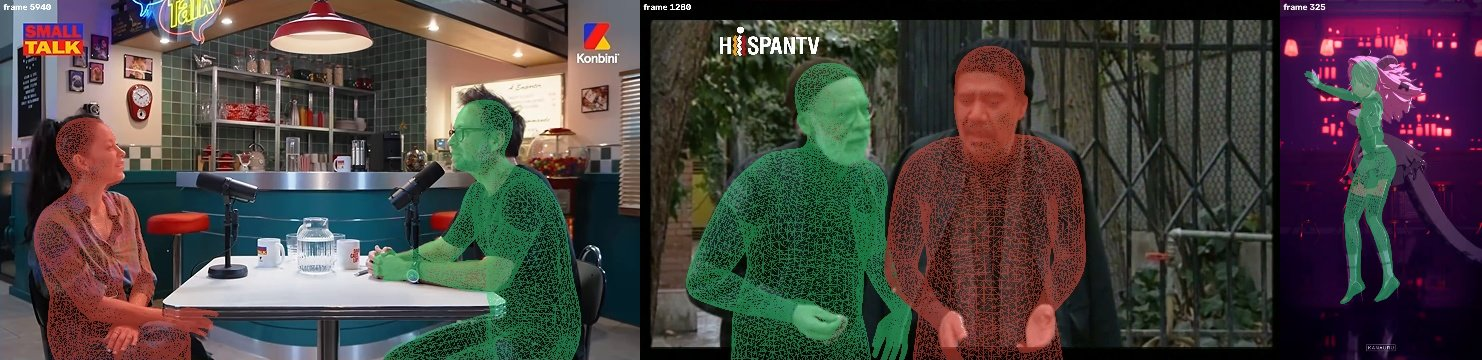
\includegraphics[width=\textwidth]{figures/sam3d_body.jpg}}{\fbox{sam3d\_body.jpg introuvable}}
\caption{Maillages SAM~3D Body projetés sur l'image, une couleur par piste SAM3 : V3 (plan large), V2 (film) et V4
(danse).}
\label{fig:sam3d}
\end{figure}

\begin{table}[H]
\centering
\caption{SAM~3D Body sur les pistes SAM3 : temps et accord des points 2D avec RTMO (une valeur par personne).}
\label{tab:sam3d-e2e}
\small
\begin{tabular}{@{}lrrrr@{}}
\toprule
Vidéo & Images & Par image & Écart médian (torse) & Points à moins de 0,2 torse \\
\midrule
V1 (une image sur 25) & 46 & 0,82~s & 0,031 & 94,8\,\% \\
V2 film & 600 & 1,05~s & 0,032 / 0,047 & 97,3 / 96,4\,\% \\
V3 talk-show & 1662 & 0,84~s & 0,031 / 0,040 & 98,2 / 93,2\,\% \\
V4 danse & 230 & 0,57~s & 0,067 & 85,0\,\% \\
\bottomrule
\end{tabular}
\end{table}

\paragraph{Par rapport à la littérature.} L'article compare SAM~3D Body aux meilleures méthodes à partir d'une image
(tableau~\ref{tab:sam3d-lit}). En 3D, il est au niveau de NLF et de CameraHMR sur 3DPW, et devant eux sur EMDB, une
base hors de son domaine d'entraînement. Le seul chiffre reproductible ici est le PCK@0,05 sur COCO, avec la boîte
annotée comme guide. Sur les 500 images de COCO val2017 déjà utilisées pour MediaPipe, on obtient 84,4, contre 86,8
dans l'article sur tout COCO val. L'écart de 2,4 points est plausible : le sous-ensemble diffère, et la normalisation
(ici, le plus grand côté de la boîte) peut différer un peu. Sur ces mêmes images, l'OKS vaut 0,894 et le PCK@0,2
0,994. MediaPipe obtenait 0,331 et 0,505, mais sans boîte (section~\ref{sec:mediapipe-tasks}) : l'écart mesure aussi
l'apport de la boîte, que SAM3 fournit dans psifx.

\begin{table}[H]
\centering
\caption{SAM~3D Body et méthodes à partir d'une image : erreurs 3D en mm (plus bas = mieux) et PCK@0,05 sur COCO
(plus haut = mieux). Chiffres de l'article \cite{sam3dbody2026}, sauf la dernière ligne, mesurée ici.}
\label{tab:sam3d-lit}
\footnotesize
\setlength{\tabcolsep}{4pt}
\begin{tabular}{@{}lrrrrrrr@{}}
\toprule
 & \multicolumn{3}{c}{3DPW} & \multicolumn{3}{c}{EMDB} & COCO \\
\cmidrule(lr){2-4}\cmidrule(lr){5-7}\cmidrule(l){8-8}
Méthode & PA-MPJPE & MPJPE & PVE & PA-MPJPE & MPJPE & PVE & PCK@0,05 \\
\midrule
HMR2.0b & 54,3 & 81,3 & 93,1 & 79,2 & 118,5 & 140,6 & 86,1 \\
CameraHMR & 35,1 & 56,0 & 65,9 & 43,3 & 70,3 & 81,7 & 80,5 \\
PromptHMR & 36,1 & 58,7 & 69,4 & 41,0 & 71,7 & 84,5 & 79,2 \\
NLF-L+fit & 33,6 & 54,9 & \textbf{63,7} & 40,9 & 68,4 & 80,6 & 74,9 \\
SAM~3D Body ViT-H & \textbf{33,2} & \textbf{54,8} & 64,1 & \textbf{38,5} & \textbf{62,9} & \textbf{74,3} & \textbf{86,8} \\
\midrule
Mesuré ici (500 images) & --- & --- & --- & --- & --- & --- & 84,4 \\
\bottomrule
\end{tabular}
\end{table}

\paragraph{Limites.}
\begin{itemize}
    \item \textbf{Image par image} : sans lissage temporel, le maillage peut trembler d'une image à l'autre (non
    mesuré à une image sur 5).
    \item \textbf{Focale par défaut} : la profondeur absolue est approximative ; la pose et la forme du corps n'en
    dépendent pas.
    \item \textbf{Coût} : 0,6 à 1~s par image, soit environ 20$\times$ le temps réel sur V3 si l'on traite toutes
    les images, du même ordre que le suivi SAM3.
    \item \textbf{Suivi} : en V3, un danseur filmé dans un encart vidéo porte le numéro de piste de l'intervieweur et
    reçoit donc son maillage. L'erreur vient du suivi SAM3.
    \item \textbf{Intégration} : les sorties (\code{.npz}) ne suivent pas encore le format des archives de pose
    psifx, et la licence SAM doit être vérifiée avant toute redistribution.
\end{itemize}

\section{Veille : solutions apparues depuis le début du travail}
\label{sec:veille}

\begin{table}[H]
\centering
\caption{Nouveautés pertinentes pour psifx, et décision.}
\label{tab:veille}
\small
\begin{tabularx}{\textwidth}{@{}lYl@{}}
\toprule
Solution & Constat & Décision \\
\midrule
SAM~3.1 \cite{hf_sam31} & Publié en mars 2026. Suivi conjoint des objets (\emph{Object Multiplex}), environ 7$\times$
plus rapide à 128 objets. Poids accessibles, mais seulement pour le code de Meta : aucune intégration
\code{transformers}. Le gain porte sur le nombre d'objets, pas sur les coupes. & À suivre \\
pyannote \code{community-1} \cite{pyannote_community1} & Remplace \code{3.1} : DER de 49,7 à 44,6\,\% sur AVA-AVD,
de 22,7 à 19,9\,\% sur AMI (chiffres de l'éditeur). Diarisation \enquote{exclusive} (un seul locuteur à la fois), qui
simplifie l'alignement avec la transcription. Demande \code{pyannote.audio} 4. & Adopté, section~\ref{sec:community1} \\
Détection du locuteur actif & Modèles entraînés, par exemple LoCoNet (95,2 mAP sur AVA) ou Light-ASD (94,1, léger)
\cite{wang2023loconet,liao2023lightasd}. Ils plafonnent encore sur des vidéos variées \cite{unitalk2025}. Pourraient
remplacer la règle sur les lèvres. & Branche à tester \\
Transcription & Canary-Qwen et Parakeet TDT v3 (multilingue) devant Whisper large-v3 sur l'Open ASR Leaderboard
\cite{open_asr_leaderboard}, mesuré surtout sur de la parole propre. & À mesurer sur nos vidéos \\
DINOv3 & Successeur de DINOv2, en accès restreint ; non testé. & Si l'accès est accordé \\
MediaPipe~1.x & L'API \enquote{Legacy Solutions} a disparu ; Holistic, Face et Pose Landmarker de l'API
\enquote{Tasks} \cite{mediapipe_holistic_tasks}. Deux fois plus rapide, mais trouve moins de visages. & Adopté,
section~\ref{sec:mediapipe-tasks} \\
SAM~3D Body \cite{sam3dbody2026} & Meta, CVPR~2026 : maillage 3D complet du corps, des mains et des pieds à partir
d'une image, guidé par des points ou des masques (donc par les masques SAM3 de psifx). Image par image, 631 à 840~M
de paramètres, accès restreint. & Testé, section~\ref{sec:sam3dbody} \\
\bottomrule
\end{tabularx}
\end{table}

% =============================================================================
\chapter{Travaux futurs}
\label{chap:futur}
% =============================================================================

\section{Optimisations non encore testées}

\begin{table}[H]
\centering
\caption{Pistes d'optimisation restantes, par modèle, classées par priorité.}
\label{tab:futur}
\small
\begin{tabularx}{\textwidth}{@{}lYl@{}}
\toprule
Modèle & Piste & Priorité \\
\midrule
\multirow{4}{*}{RTMPose} & Inférer toutes les personnes en un seul batch (\code{rtmlib} appelle le modèle une fois par personne) & Haute \\
& Détecter une image sur N et suivre les boîtes entre deux détections & Haute \\
& TensorRT (fp16, puis INT8 sur Tensor Cores) \cite{ort_tensorrt} & Haute \\
& IOBinding et CUDA graphs \cite{ort_cuda,optimum_gpu} ; preset \code{lightweight} & Moyenne \\
\midrule
\multirow{4}{*}{RTMO} & TensorRT fp16 (le modèle représente presque tout le temps de calcul) & Haute \\
& Traiter plusieurs images vidéo par appel (dimension batch dynamique) & Haute \\
& IOBinding, CUDA graphs ; prétraitement sur GPU ; tailles S et L & Moyenne \\
& TensorRT INT8 avec calibration soignée & Moyenne \\
\midrule
\multirow{4}{*}{ViTPose} & Détecteur plus léger (45\,\% du temps) & Haute \\
& Détecter une image sur N et suivre les boîtes & Haute \\
& Prétraitement sur GPU (22\,\% du temps) & Haute \\
& \code{torch.compile} à formes fixes avec cache ; ViTPose++ ; TensorRT ; INT8 via \code{torchao} & Moyenne à basse \\
\midrule
\multirow{4}{*}{DETRPose} & Pont efficace : images brutes en mémoire au lieu de PNG & Haute \\
& Sous-processus persistant (pas de rechargement ni de recompilation par vidéo) & Haute \\
& Prétraitement sur GPU ; tester DETRPose avec le numpy de psifx & Haute à moyenne \\
& Export TensorRT fourni par le dépôt ; tailles N, S, L & Moyenne \\
\bottomrule
\end{tabularx}
\end{table}

Distillation, élagage et quantification avec ré-entraînement restent hors de portée à court terme
(section~\ref{sec:sota-optim}).

\section{Axes d'amélioration retenus}

Trois axes ont été retenus pour la phase suivante :
\begin{enumerate}
    \item \textbf{Corps entier} : RTMW \cite{jiang2024rtmw}, de la même famille et avec la même dépendance que RTMO,
    pour retrouver le visage et les mains que les modèles COCO-17 ne fournissent pas, contrairement à MediaPipe
    Holistic.
    \item \textbf{Multi-personnes natif} : produire une archive par personne détectée, avec un suivi d'identité entre
    images, sans exiger les masques SAM3.
    \item \textbf{Occlusion et SAM~3.1} : évaluer la robustesse à l'occlusion mutuelle (CrowdPose, ou occlusion
    volontaire sur \code{Video.mp4}) et envisager DEKR si le besoin se confirme \cite{geng2021dekr} ; passer à
    SAM~3.1 dès son support dans \code{transformers}, en testant d'ici là un re-prompting autour de SAM3
    \cite{pvuw2026reprompt}.
\end{enumerate}

Le test d'occlusion a été fait avec OCHuman (section~\ref{sec:phase2-reunion}). Au 27 octobre 2026, SAM~3.1 n'est
toujours pas intégré à \code{transformers} (section~\ref{sec:veille}). Le test de bout en bout
(section~\ref{sec:e2e}) ajoute les axes suivants, tournés vers la fiabilité sur des vidéos réelles et bruitées :
\begin{enumerate}[resume]
    \item \textbf{Association voix--personne dans psifx} : faire du script par les lèvres une commande
    (\code{psifx audio identification}) au même format que l'identification par micros, puis la comparer à un modèle
    de détection du locuteur actif entraîné \cite{liao2023lightasd}.
    \item \textbf{Association robuste aux petits groupes de voix} : quand la diarisation coupe une personne en deux,
    le petit groupe doit rejoindre la personne la plus proche plutôt que basculer \enquote{hors champ}
    (section~\ref{sec:mediapipe-tasks}). Corriger aussi l'identification par micros, qui plante quand la diarisation
    trouve plus de locuteurs que de micros, ou avec le modèle speechbrain par défaut (section~\ref{sec:dev-run}).
    \item \textbf{Visage avec MediaPipe \enquote{Tasks}} : retrouver les visages manqués sans dégrader le signal des
    lèvres, par exemple en ne gardant que les visages assez grands et de face.
    \item \textbf{Maillage 3D du corps} : SAM~3D Body (section~\ref{sec:sam3dbody}) reste à mesurer sur une vérité
    terrain 3D (3DPW ou EMDB), à lisser dans le temps, puis à intégrer comme commande psifx écrivant les archives de
    pose habituelles ; le maillage pourrait remplacer le squelette 3D de MediaPipe dans la vidéo reconstruite.
    \item \textbf{Robustesse au bruit et à la musique} : séparation de la voix avant transcription (option psifx),
    transcription vide plutôt qu'un plantage quand aucune parole n'est détectée, et mesure du WER sur de la parole
    bruitée.
    \item \textbf{Coût du suivi} : SAM3 domine le temps de calcul (13 à 19$\times$ le temps réel) ; mesurer
    SAM~3.1 dès qu'il est utilisable, et une détection une image sur N.
\end{enumerate}

Restent en réserve : les optimisations de vitesse vidéo du tableau~\ref{tab:futur}, une nouvelle mesure de DETRPose
avec synchronisation CUDA et de toutes les vitesses sur un GPU non partagé, et la validation de la licence de
Sapiens2 avant tout nouvel investissement.

% =============================================================================
\chapter{Conclusion}
% =============================================================================

Ce travail a établi, mesures à l'appui, que le backend de pose actuel de psifx est très largement dépassé en
précision par plusieurs modèles récents sous licence compatible. Quatre d'entre eux (RTMPose, RTMO, ViTPose,
DETRPose) sont désormais intégrés à psifx comme remplaçants directs de MediaPipe, avec des tests unitaires, un
test de non-régression de précision sur COCO et un outillage de mesure partagé entre branches. Aucun modèle ne
domine sur toutes les dimensions : ViTPose ou RTMPose pour la précision, RTMO pour le compromis
vitesse/simplicité, en particulier en fp16 (110 images/s sans perte de précision).

Les mesures d'optimisation rappellent qu'un gain annoncé sur un modèle ne se traduit pas forcément de bout en
bout : il faut profiler la chaîne complète avant d'optimiser, et vérifier la précision après chaque optimisation.
RTMO et ViTPose ont été retenus pour la bibliothèque (section~\ref{sec:decisions}) ; la phase suivante porte sur le
corps entier, le multi-personnes natif et l'occlusion (chapitre~\ref{chap:futur}).

La seconde phase a montré que psifx, complété par quelques scripts, va de la vidéo brute à des données
exploitables : poses 2D et 3D par personne, transcription et sous-titres attribués à chaque personne, réutilisés pour
reconstruire une vidéo. Elle a surtout montré où cette chaîne casse sur des vidéos réelles : le montage, que le suivi
SAM3 gère désormais par plan avec une ré-identification par l'apparence ; la musique, qui demande de séparer la voix ;
les visages peu lisibles et la diarisation qui sur-découpe. La suite vise la fiabilité dans ces conditions : intégrer
l'association voix--personne à psifx en la rendant robuste aux erreurs de diarisation, et agir avant la diarisation
pour le bruit fort (chapitre~\ref{chap:futur}). Les outils ont été modernisés en chemin : pyannote \code{community-1},
qui estime bien mieux le nombre de locuteurs dans le bruit et sur les films, et MediaPipe \enquote{Tasks}, deux fois
plus rapide. Enfin, SAM~3D Body, guidé par les masques SAM3, apporte un maillage 3D complet du corps, que la
bibliothèque d'origine ne fournissait pas, avec une précision 2D proche de celle annoncée dans l'article. Tout est
rassemblé sur \code{dev} et validé dans un environnement neuf, prêt pour une version de \code{main}.

% =============================================================================
\appendix
\chapter{Reproduction}
% =============================================================================

\section{Branches}

\begin{table}[H]
\centering
\footnotesize
\begin{tabular}{@{}ll@{}}
\toprule
Branche & Contenu \\
\midrule
\code{dev} & Recherche, banc, tests, base COCO-17, aides ONNX, mesure \\
\code{feature/pose-rtmpose} & \code{psifx video pose rtmpose} \\
\code{feature/pose-rtmo} & \code{psifx video pose rtmo} \\
\code{feature/pose-vitpose} & \code{psifx video pose vitpose} \\
\code{feature/pose-detrpose} & \code{psifx video pose detrpose} \\
\code{optim/rtmpose-fp16-int8} & \code{--precision fp16|int8} \\
\code{optim/rtmo-fp16-int8} & \code{--precision fp16|int8} \\
\code{optim/vitpose-compile-fp16} & \code{--fp16}, \code{--compile} \\
\code{optim/detrpose-compile-fp16} & \code{--fp16}, \code{--compile} \\
\code{analysis/vitpose-gap} & Analyse de l'écart de ViTPose \\
\code{analysis/int8-root-cause} & Analyse de l'échec de l'INT8 \\
\code{feature/pose-body-command} & \code{psifx video pose body} (RTMO, ViTPose) \\
\code{feature/tests-ochuman} & Test de précision sur OCHuman \\
\code{fix/sam3-shot-changes} & Suivi SAM3 à travers les plans (mergée dans \code{dev}) \\
\code{experiment/e2e-demo} & Test de bout en bout, 3D MediaPipe (mergée dans \code{dev}) \\
\code{feature/diarization-community-1} & pyannote~4, \code{community-1} (mergée dans \code{dev}) \\
\code{feature/mediapipe-tasks} & MediaPipe \enquote{Tasks} (mergée dans \code{dev}) \\
\code{fix/numpy-skvideo}, \code{fix/e2e-*} & Correctifs trouvés par l'environnement neuf (mergées) \\
\code{dev-before-integration} & \code{dev} avant l'intégration du 27 octobre (sauvegarde) \\
\code{feature/sam3d-body} & Maillage 3D SAM~3D Body sur les pistes SAM3 (mergée dans \code{dev}) \\
\bottomrule
\end{tabular}
\end{table}

\section{Commandes}

Banc de recherche (\code{research/benchmark/}) :
{\footnotesize
\begin{verbatim}
python prepare_coco_subset.py --n 50
python run_accuracy.py --backends mediapipe,rtmpose,vitpose,rtmo,detrpose
python run_video_benchmark.py --backends mediapipe,rtmpose,vitpose,rtmo,detrpose
python aggregate_results.py
\end{verbatim}
}

Intégrations et optimisations :
{\footnotesize
\begin{verbatim}
pytest tests/unit
pytest tests/integration/video/test_pose_coco_accuracy.py -s
python run_psifx_cli_benchmark.py --tool rtmo \
    --extra="--device cuda --precision fp16"
python time_psifx_pose.py --tool rtmo --device cuda \
    --kwargs '{"precision": "fp16"}'
python compare_psifx_cli.py
\end{verbatim}
}

Test OCHuman et test de bout en bout :
{\footnotesize
\begin{verbatim}
OCHUMAN_ROOT=/path/to/ochuman pytest -m dataset -s
python research/e2e/run_pipeline.py .e2e_outputs/v3_talkshow --chunk_size 64
python research/e2e/summarize.py .e2e_outputs/v1_example .e2e_outputs/v2_ava ...
\end{verbatim}
}

\section{Versions logicielles}

Environnement de \code{dev} au 27 octobre 2026 (installé de zéro) : PyTorch 2.8.0 (cu128), \code{transformers} 5.3.0
(SAM3, DINOv2-small), huggingface-hub 1.7.1, \code{rtmlib} 0.0.16, \code{onnxruntime-gpu} 1.20.2, mediapipe 1.1.1
(API \enquote{Tasks}), pyannote.audio 4.0.7 (\code{community-1}), whisperx 3.8.7rc1, torchcodec 0.7.0, numpy 2.2.6,
protobuf 7.36.2. Les mesures des chapitres~\ref{chap:resultats}~et suivants, avant la section~\ref{sec:mediapipe-tasks},
ont été faites avec mediapipe 0.10.14, protobuf 4.25.9, numpy 2.0.2 et pyannote.audio 3.3.2. Environnement DETRPose : Python
3.11.9, PyTorch 2.14.1 (cu130), numpy 1.23.5.

\printbibliography[heading=bibintoc, title={Bibliographie}]

\end{document}
